

\documentclass[
    left=2.5cm,         % Sadly, generic margin parameter
    right=2.5cm,        % doesnt't work, as it is
    top=2.5cm,          % superseded by more specific
    bottom=3cm,         % left...bottom parameters.
    bindingoffset=6mm,  % Optional binding offset.
    nohyphenation=false % You may turn off hyphenation, if don't like.
]{eiti/eiti-thesis}

\langpol % Dla języka angielskiego mamy \langeng
\graphicspath{{img/}}             % Katalog z obrazkami.
\addbibresource{bibliografia.bib} % Plik .bib z bibliografią

\begin{document}


\EngineerThesis % Dla pracy inżynierskiej mamy \EngineerThesis
\instytut{Instytut Mikroelektroniki i Optoelektroniki }
\kierunek{Elektronika i Telekomunikacja}
\specjalnosc{Inżynieria Komputerowa}
\title{
    Zastosowanie wybranych algorytmów uczenia maszynowego w zarządzaniu łańcuchem dostaw \\
    Application of selected machine learning algorithms in supply chain management
}
\engtitle{ % Tytuł po angielsku do angielskiego streszczenia
    Application of selected machine learning algorithms in supply chain management \\
    difficult to read, understand and pronounce
}
\author{Jarosław Wanczewski}
\album{309470}
\promotor{Marek Niewiński}
\date{\the\year}
\maketitle



\cleardoublepage % Zaczynamy od nieparzystej strony
\begin{abstract}


%\begin{abstract}
To jest moje streszczenie. Moja praca dotyczy...
%\end{abstract}
%\documentclass{article}
%\usepackage[utf8]{inputenc}
%\title{Tytuł Twojego Dokumentu}
%\author{Twoje Imię i Nazwisko}
%\date{\today}

%\begin{document}

%\maketitle
%\section{Wprowadzenie}
%Lorem ipsum dolor sit amet, consectetur adipiscing elit. Integer ac quam non neque dictum consequat.

%\section{Rozwinięcie}
%Lorem ipsum dolor sit amet, consectetur adipiscing elit. Integer ac quam non neque dictum consequat.

%\end{document}





\end{abstract}
\clearpage % Zakończ streszczenie i rozpocznij resztę dokumentu


%--------------------------------------
% Oświadczenie o autorstwie
%--------------------------------------
\cleardoublepage  % Zaczynamy od nieparzystej strony
\pagestyle{plain}
\makeauthorship

%--------------------------------------
% Spis treści
%--------------------------------------
\cleardoublepage % Zaczynamy od nieparzystej strony
\tableofcontents

%--------------------------------------
% Rozdziały
%--------------------------------------
\cleardoublepage % Zaczynamy od nieparzystej strony
\pagestyle{headings}

\newpage % Rozdziały zaczynamy od nowej strony.
\section{Wstęp}




\subsection{Tło}

Współczesny świat (postepujaca globalizacja) charakteryzuje się dynamicznymi zmianami, rosnącą konkurencją oraz rosnącym zapotrzebowaniem na coraz bardzo skomplikowane usługi i produkty, stawia to przed przedsiębiorstwami wiele wyzwań związanych z efektywnym zarządzaniem łańcuchem dostaw. 

W szczególności kluczowe technologie mają ogromne znaczenie w długoterminowej perspektywie konkurencyjności firm. Dlatego warto rozważyć ich zastosowanie. Współczesne kluczowe technologie XXI wieku znane są jako sztuczna inteligencja (AI). Analogicznie do ludzkiego poznania, termin "sztuczna inteligencja" obejmuje systemy zdolne do przetwarzania informacji, rozumienia języka, wykonywania działań i skoncentrowania się na celach, a także zdobywania wiedzy do rozwiązywania problemów, przy wykorzystaniu uczenia maszynowego. Aby wykorzystać tę zdolność uczenia się przez system, uczenie maszynowe (ML) wyłoniło się jako niezależna dziedzina badań i technologii w kontekście sztucznej inteligencji. W odróżnieniu od ręcznego kodowania pojedynczych rozwiązań, takich jak korzystanie z reguł czy ontologii, wiedza z zakresu uczenia maszynowego jest automatycznie dostarczana przez odpowiednie systemy, które wykorzystują algorytmy oparte na empirycznych danych do rozwiązywania problemów.\cite{Weinke2023}


 Sztuczna inteligencja jest obecnie jedna z najszybciej rozwijających sie technik, mającą w sobie potencjał do przełomowego wpływu na sposób organizacji i funkcjonowania zarówno społeczeństwa jako całości, jak i pojedynczych osób.Juz obecnie widzimy oddziaływanie SI na gospodarke, w szczególnosci na produkcje przemyslową, gdzie tzw. przemysł 4.0, oparty na szerokiej robotyzacji zastepuje tradycyjne formy wytwarzania produktów.\cite{Nowak2022}


\subsection{Opis problemu}
   Dawniej począwszy od kadry kierowniczej wyższego szczebla po kadrę kierowniczą pierwszej linii,  mierzac się ze złożonymi i krytycznymi decyzjami to tradycyjnie takie decyzje zależały od ich doświadczenia i osądu.Jednakże rynek przestawił się na krótkie serie produkcyjne, aby zaspokoić szybko zmieniający się popyt, a koszty zostały obniżone na rzecz metod produkcji „dokładnie na czas”. decyzje stały się bardziej złożone. Jednocześnie procesy operacyjne (produkcja) staje sie bardziej zautomatyzowana i zintegrowana, co umożliwi większą kontrolę nad łańcuchem dostaw. Dlatego ostatnio coraz większą uwagę poświęca się technikom sztucznej inteligencji (AI).\cite{Wong2013}
   
   W dobie rozwijającej się i powszechnie dostępnej technologii oraz 
dostępu do aktualnej informacji nie wystarczy oferować wyroby i usługi w tzw. ,,standardzie”. 
Wyróżniać się wśród konkurencji, to znaczy działać nieszablonowo, oferować wyroby i usługi 
dedykowane, ,,szyte na miarę” pod indywidualne potrzeby klientów, przy zachowaniu 
wymaganego poziomu jakości. \cite{Jozwiak2017}

    Łańcuch dostaw to obszar istotny , który ma wpływ na  konkurencyjność, elastyczność i zdolność do czestego i szybkiego dostosowywania się do coraz szybciej zmieniającego sie rynku. W ten obszar doskonale wkomponowuja sie  technologie z zakresu uczenia maszynowego które staja się znaczącym narzędziem wspierającym lub całkowicie decydujacym w zarządzaniu łańcuchem dostaw.W dzisiejszym środowisku biznesowym, które cechuje się rosnącą ilością dostępnych danych oraz coraz bardziej złożonymi danymi, algorytmy uczenia maszynowego zaczynają stanowić kluczowy element umożliwiający  podejmowanie bardziej poinformowanych decyzji, redukcję kosztów oraz zwiększenie efektywności operacyjnej.
    
    Biorąc pod uwagę złożoność zadań planowania, zarządzania i kontroli w przemysłowych łańcuchach wartości, aplikacje ML uznawane są za niezwykle istotne dla wspierania i autonomicznej realizacji logistycznych procesów decyzyjnych\cite{Weinke2023}
    
\subsection{Cele}
Celem jest zbadanie i ocena potencjału zastosowania wybranych algorytmów uczenia maszynowego w zarządzaniu łańcuchem dostaw. 
\subsection{Zakres badania}
Praca skupia się na analizie, projektowaniu oraz implementacji algorytmów uczenia maszynowego w różnych częsciach zarządzania łańcuchem dostaw, takich jak prognozowanie popytu, planowanie produkcji, zarządzanie zapasami .
        
\newpage % Rozdziały zaczynamy od nowej strony.
\section{Przeglad }
W rozdziale tym dokonuje przeglądu istotnych zagadnień związanych z zarządzaniem łańcuchem dostaw oraz uczeniem maszynowym. Przedstawimy definicje, teorie, rodzaje  zarządzania łańcuchem dostaw  i maszynowego uczenia . Następnie omówiam definicje i zastosowania maszynowego uczenia w zarządzaniu łańcuchem dostaw.


\subsection{Zarządzanie łańcuchem dostaw}
W niniejszym podrozdziale dokładnie omówiam najważniejsze zagadnienia związane z zarządzaniem łańcuchem dostaw( definicje, cele oraz znaczenie) . Ponadto wyjaśniam z jakich elementów składa się zarządzanie łańcuchem dostaw.

\vspace{\baselineskip}
\subsubsection{Teoria Zarządzania Łańcuchem Dostaw} 
\vspace{\baselineskip}
\textbf{Wyjaśnienie Zarządzania Łańcuchem Dostaw }

Zarządzanie łańcuchem dostaw (ang. Supply Chain Management, SCM) jest kompleksowym podejściem do planowania, kontrolowania i monitorowania wszystkich procesów związanych z dostarczaniem produktów lub usług od dostawców do klientów końcowych. Jest to obszar, który obejmuje wiele etapów, począwszy od zaopatrzenia, produkcji, dystrybucji, aż po dostarczenie produktu lub usługi do ostatecznego użytkownika.

Zarządzanie łańcuchem dostaw (ang. Supply Chain Management – SCM) – zarządzanie przepływami między ogniwami łańcuchem dostaw. Umożliwia projektowanie, planowanie, realizację, kontrolę oraz monitoring łańcucha dostaw. \cite{wik2023}



Wg. Encyklopedii zarzadzania Łańcuch dostaw - obejmuje wszelkie czynności związane z transportem oraz przeróbką towarów, wspominając tutaj również o początkowym etapie, czyli pozyskiwaniu wszelkiego rodzaju surowców oraz etapie końcowym tj. dostarczeniu produktu konsumentom. Pojęcie to zawiera również przepływ informacji, które są istotne podczas całego procesu. \cite{zarz2023}

Zarządzanie łańcuchem dostaw obejmuje wszystkie działania, które przekształcają surowce w gotowe produkty i oddają je w ręce klientów. Może to obejmować określanie źródła dostaw, projektowanie, produkcję, magazynowanie, wysyłkę i dystrybucję. Celem SCM jest poprawa wydajności, jakości, produktywności i zadowolenia klientów. \cite{scm2023}

Łańcuch dostaw jest to skoordynowana sieć wzajemnych powiązań logistyczno - operacyjnych, która obejmuje wszelkie firmy, obiekty i działania biznesowe zaangażowane w pozyskiwanie, opracowywanie, wytwarzanie i dostarczanie produktów.
Każda firma tworzy swój własny łańcuch dostaw, aby móc wytwarzać produkty i wprowadzać je na rynek. Może również sama być ogniwem w łańcuchach dostaw innych firm. Działania łańcucha dostaw przekształcają zasoby naturalne, surowce i komponenty w gotowy produkt, który jest dostarczany do użytkownika końcowego. \cite{wdx2023}

 (SCM) zajmuje się systemem zakupów (zakup surowców/komponentów), zarządzaniem operacyjnym (zapewnienie produkcji wysokiej jakości produktów z dużą szybkością, dobrą elastycznością i niskimi kosztami produkcji), logistyką i kanałami marketingowymi , dzięki któremu surowce można przekształcić w gotowe produkty i dostarczyć klientom końcowym.Węższa definicja zarządzania łańcuchem dostaw to „projektowanie, planowanie, realizacja, kontrola i monitorowanie działań w łańcuchu dostaw w celu tworzenia wartości netto, budowania konkurencyjnej infrastruktury, wykorzystania światowej logistyki, synchronizacji podaży z popytem i pomiaru wydajności globalnie”. Może to obejmować przemieszczanie i przechowywanie surowców, zapasów w toku, wyrobów gotowych i kompleksową realizację zamówień od punktu pochodzenia do punktu konsumpcji. \cite{wiken2023}

\vspace{\baselineskip}
\textbf{Historia}

Łańcuchy dostaw istnieją od czasów starożytnych, poczynając od pierwszego wytworzonego i sprzedanego produktu. Wraz z nadejściem industrializacji zarządzanie łańcuchem dostaw stało się bardziej złożone i pozwoliło przedsiębiorstwom na efektywniejsze wytwarzanie i dostarczanie towarów i usług. Na przykład wprowadzona przez Henry'ego Forda standaryzacja części samochodowych okazała się przełomem, który pozwolił na masową produkcję towarów, aby sprostać wymaganiom rosnącej liczby klientów. Z biegiem czasu kolejne zmiany (takie jak wprowadzenie na rynek komputerów) systematycznie zwiększały poziom zaawansowania systemów SCM. Systemy te pozostawały jednak przez wiele lat zasadniczo liniową, autonomiczną funkcją zarządzaną przez specjalistów ds. łańcucha dostaw. 
Sytuacja zmieniła się diametralnie wraz z pojawieniem się Internetu, innowacji technologicznych i gospodarki globalnej opartej na popycie. Obecnie zarządzanie łańcuchem dostaw nie jest już funkcją liniową, ale raczej złożonym zbiorem niejednorodnych sieci dostępnych całodobowo. W centrum tych sieci znajdują się konsumenci oczekujący realizacji swoich zamówień w wybrany przez nich sposób.\cite{oracle2023}

\vspace{\baselineskip}
\textbf{Pochodzenie terminu}.

W 1982 roku Keith Oliver, konsultant w firmie Booz Allen Hamilton, w wywiadzie dla Financial Times wprowadził do domeny publicznej termin „zarządzanie łańcuchem dostaw”. W 1983 roku WirtschaftsWoche w Niemczech opublikowało po raz pierwszy wyniki wdrożonego tzw. „projektu zarządzania łańcuchem dostaw”, kierowanego przez Wolfganga Partscha.
W połowie lat 90. termin „zarządzanie łańcuchem dostaw” zyskał na popularności, gdy ukazała się lawina artykułów i książek na ten temat. Pierwotnie łańcuchy dostaw zdefiniowano jako obejmujące wszystkie działania związane z przepływem i przetwarzaniem towarów od surowców do użytkownika końcowego lub konsumenta końcowego, a także powiązane przepływy informacji. Mentzer i in. uważają za godne odnotowania, że te wcześniejsze definicje obejmowały konsumenta końcowego. Zarządzanie łańcuchem dostaw zostało następnie zdefiniowane jako integracja działań w łańcuchu dostaw poprzez ulepszone relacje w łańcuchu dostaw w celu osiągnięcia przewagi konkurencyjnej. \cite{wiken2023}


\vspace{\baselineskip}
\subsubsection{Cele Zarządzania Łańcuchem Dostaw}



Najczęściej opisywanymi celami łańcucha dostaw w ujęciu logistycznym jest:

  \par - Minimalizacja kosztów wynikających z przepływu towarów i informacji przy zachowaniu dobrego poziomu obsługi klienta
  
  \par - Krótki czas realizacji zamówień oraz bezproblemowość i elastyczność dostaw
  
   \par- Optymalizacja poziomu zapasów wraz z dostosowaniem się do potrzeb rynku \cite{zarz2023}


Podsumowujac: Głównym celem zarządzania łańcuchem dostaw jest zapewnienie, że produkty lub usługi są dostarczane w odpowiednim czasie, w optymalnych ilościach, przy minimalnych kosztach oraz z zachowaniem wysokiej jakości. SCM dąży do zintegrowania wszystkich elementów łańcucha dostaw, tak aby procesy były bardziej efektywne i konkurencyjne.

Ale wazne aby odnotować zmiane w celach , ktore cele sa obecnie najwazniejsze:
 Dzisiejsze systemy SCM są całkowicie ukierunkowane na klienta.
Celem zarządzania łańcuchem dostaw zawsze było zwiększanie efektywności i obniżanie kosztów. Cele te nie uległy zmianie, ale obecnie główną rolę w ustalaniu priorytetów takiego zarządzania odgrywa klient. Mówi się, że „doświadczenia klientów żyją i umierają w łańcuchu dostaw”.
Lojalność klientów zależy od tego, czy przedsiębiorstwo jest w stanie szybko i dokładnie spełnić ich oczekiwania. Dostawy surowców, produkcja, logistyka, sprzedaż i zarządzanie zamówieniami muszą być ze sobą skoordynowane, aby klient otrzymał to, co chce, w rozsądnym terminie. W tym celu przedsiębiorstwo musi analizować swoje łańcuchy dostaw z perspektywy klientów. Nie chodzi tu bowiem tylko o terminową dostawę, ale również o wykonanie we właściwym czasie wszystkich niezbędnych czynności, zarówno przed taką dostawą, jak i w jej trakcie oraz po jej zrealizowaniu.\cite{oracle2023}


\vspace{\baselineskip}
\subsubsection{Znaczenie zarządzania Łańcuchem Dostaw}

Łańcuchy dostaw zawsze były napędzane przez wiele sił globalnych i politycznych, a nawet przez warunki pogodowe i wydarzenia naturalne. Jest jednak jedna rzecz, która jest pewna w zarządzaniu łańcuchem dostaw i to jest zmiana. 
Nowoczesna logistyka stawia menedżerów przed wieloma wyzwaniami skutecznej organizacji łańcuchów dostaw, optymalizacji kosztów i zarządzania stanami magazynowymi. Wszystko to ułatwią rozwijające się technologie Łańcuchów Dostaw 4.0. To szerokie pojęcie obejmuje między innymi zastosowanie IoT w logistyce, użycie zaawansowanej robotyki w magazynach oraz zaawansowaną analizę Big Data, a nawet sztuczną inteligencję. Dzięki czujnikom, sieciom, nowoczesnemu oprogramowaniu i automatyzacji możliwe jest nie tylko zwiększenie skuteczności procesów logistycznych, ale także ograniczenie kosztów oraz wyższy poziom zadowolenia klienta z dostaw.
Znaczenie systemów SCM: Istota zarządzania łańcuchem dostaw
Wystarczy się rozejrzeć. Wszystko, co znajduje się w domu lub zakładzie pracy, trafiło tu dzięki łańcuchom dostaw. Działania te wymagają zaangażowania pracowników z milionów miejsc pracy na całym świecie. Przez łańcuch dostaw przewija się wszystko — od tanich dóbr konsumpcyjnych aż po przyrządy chirurgiczne i kluczowe zasoby. Wciąż jednak, mimo iż zarządzanie łańcuchami dostaw leży u podstaw gospodarki światowej, wiele organizacji korzysta w tym celu z procesów i maszyn stosowanych od 50 lat.\cite{scm2023}

  Wiele firm po prostu przestałoby działać bez zarządzania łańcuchem dostaw, więc to dość duże korzyści SCM.  Niektóre z zalet zoptymalizowanego zarządzania łańcuchem dostaw obejmują: 

   - Większa produktywność: systemy do zarządzania zasobami przedsiębiorstwa i przeglądy zapobiegawcze zwiększają wydajność maszyn i systemów. Może to pomóc w wyeliminowaniu wąskich gardeł, usprawnieniu procesów i zwiększeniu produktywności. Zautomatyzowane procesy i responsywne analizy danych przekładają się na szybszy transport i krótszy czas dostawy.
   
   -Niższe koszty łańcucha dostaw: przy użyciu analiz predykcyjnych można wyeliminować konieczność szacowania w oparciu o przypuszczenia. Pozwoli to ograniczyć zarówno marnotrawienie zapasów, jak i ryzyko ich deficytu. Internet rzeczy zapewnia większą responsywność istniejących zasobów oraz maksymalnie wydajny i praktyczny przepływ pracy w każdej sytuacji. Bardziej precyzyjne prognozy umożliwiają ponadto redukcję liczby niezaładowanych w pełni samochodów dostawczych i nieskoordynowanych tras dostaw, a także bardziej efektywne zarządzanie flotą.
   
   - Większa elastyczność i odporność łańcucha dostaw: Trendy i zmiany na rynku mogą nastąpić nagle. Odporne systemy SCM są elastyczne, aby dostosować się do każdej sytuacji. Dane w czasie rzeczywistym i inteligentne analizy mogą pomóc menedżerom łańcucha dostaw przenieść maszyny i personel do lepszych przepływów pracy. Opinie klientów można od razu usłyszeć i podjąć odpowiednie działania. Wirtualne zapasy i inteligentne procesy magazynowe zapewniają dostosowanie podaży i popytu.
   
   -Wyższa jakość produktów: zapewnienie zespołom ds. badań i rozwoju dostępu do informacji zwrotnych od klientów sprawia, że podczas projektowania i opracowywania produktów brane są pod uwagę ich potrzeby. Zarówno zespół ds. badań i rozwoju, jak i zespół ds. produkcji mogą wykorzystać informacje dostępne dzięki uczeniu maszynowemu i analizom, aby reagować na trendy i oczekiwania klientów oraz doskonalić projekty produktów.
    
    -Lepsza obsługa klienta: najlepsze praktyki SCM są zorientowane na klienta i zaprojektowane tak, aby były responsywne i adaptacyjne. Dzięki konkurencji tylko jednym kliknięciem, nowoczesny SCM pozwala firmom wdrażać opinie klientów i trendy, umożliwiając zarówno mikrorealizację, jak i personalizację na dużą skalę.
    
    -Większa przejrzystość i zrównoważony rozwój: SCM umożliwia pełną przejrzystość, od etapu projektowania i produkcji po logistykę, dostawę i zwroty. Dzięki możliwości wglądu we wszystkie dane wejściowe i wyjściowe w całym łańcuchu organizacje mogą znacznie poprawić swój wpływ na środowisko, często współpracując w tym celu bezpośrednio z dostawcami i innymi dostawcami. \cite{scm2023}

 

\vspace{\baselineskip}
\subsubsection{Składniki Efektywnego Zarządzania Łańcuchem Dostaw}


\paragraph{Elementy łańcucha dostaw}


Istnieje pięć elementów tradycyjnych systemów zarządzania łańcuchem dostaw:

    -Planowanie. Planowanie i zarządzanie wszystkimi zasobami wymaganymi do zaspokojenia zapotrzebowania klientów na produkt lub usługę firmy. Po ustanowieniu łańcucha dostaw należy określić mierniki, które pozwolą zmierzyć czy łańcuch dostaw jest wydajny, efektywny, zapewnia wartość klientom i spełnia cele firmy.
    
   - Zaopatrzenie. Wybór dostawców kwalifikowanych, którzy zapewnią towary i usługi potrzebne do stworzenia produktu. Należy również ustalić procesy monitorowania i zarządzania relacjami z dostawcami. Kluczowe działania w tych procesach obejmują zamawianie, przyjmowanie, zarządzanie stanami magazynowymi oraz realizację płatności dla dostawców.
    
   - Produkcja. Czynności wymagane do przyjęcia surowców, wytworzenia produktu, badania jakości, opakowania do wysyłki i przygotowania harmonogramu dostaw.
    
   - Dostawa i logistyka. Koordynacja zamówień klientów, magazynowanie, planowanie dostaw, wysyłka towarów, wystawianie faktur i odbieranie płatności.
    
   - Zwroty. Stworzenie procesu odbioru wadliwych, nadmiarowych lub niechcianych produktów\cite{wdx2023}



Aleksander Wielki powiedział kiedyś słynnie: „Moi logistycy nie mają poczucia humoru… ponieważ wiedzą, że jeśli moja kampania się nie powiedzie, są pierwszymi, których zabiję”. I choć ten przykład jest trochę skrajny, niemniej jednak ilustruje on, jak ważne dla cywilizacji ludzkiej były zawsze łańcuchy dostaw. Efektywne i odporne narzędzia i praktyki w zakresie zarządzania łańcuchem dostaw są niezbędnym elementem przetrwania i sukcesu firmy. Niektóre z podstawowych procesów SCM obejmują:   

    -Planowanie łańcucha dostaw to proces przewidywania popytu na produkty i koordynowania powiązań w łańcuchu dostaw w celu jego realizacji. Oprócz prognozowania popytu i planowania obejmuje on planowanie dostaw, planowanie potrzeb materiałowych (MRP), planowanie produkcji, planowanie sprzedaży i produkcji (SOP)i inne. 

   - Zarządzanie cyklem życia produktu  to proces zarządzania produktem przez cały jego cykl życia – od pomysłu, inżynierii i projektowania po produkcję, serwis i utylizację (lub recykling).

    -Nabycie to proces nabywania materiałów, towarów i usług w celu zaspokojenia potrzeb biznesowych i zapewnienia jakości, uczciwej ceny i wartości tych towarów. Głównym wyzwaniem dla zaopatrzenia i określania źródła dostaw jest przewidywanie dokładnych wolumenów zamówień, ponieważ zarówno niedobory, jak i nadwyżki mogą być szkodliwe dla firmy. 

   - Zarządzanie logistyką to transport i składowanie towarów od początku łańcucha dostaw, z surowcami i produkcją, po dostawę gotowych produktów do sklepów lub klientów – a nawet do obsługi produktów, zwrotów i recyklingu. Funkcje biznesowe obejmują zarządzanie transportem przychodzącym i wychodzącym, zarządzanie flotą, gospodarkę magazynową, kontrolę zapasów i obsługę klienta. 

   - Zarządzanie realizacją produkcji (MES) monitoruje, śledzi, dokumentuje i kontroluje proces wytwarzania towarów. Utrzymuje produkcję i procesy tak szczupłe, jak to tylko możliwe – zachowując (i poprawiając) jakość, zrównoważony rozwój i zadowolenie klientów. 

   - Zarządzanie aktywami przedsiębiorstwa to proces zarządzania aktywami fizycznymi i ich utrzymania w całym łańcuchu dostaw, od robotyki fabrycznej po floty dostaw. Czujniki IoT, łączność maszyna-maszyna (M2M)– poprawiają wydajność, czas pracy, bezpieczeństwo oraz prewencyjną i predykcyjną konserwację. Niektóre połączone zasoby mogą nawet przewidywać naprawy lub awarie i samodzielnie przeprowadzać konserwację — bezpośrednio do określania źródła dostaw i zamawiania części potrzebnych do wydłużenia cyklu życia.\cite{scm2023}






\subsection{Maszynowe Uczenie}

W tym rozdziale omawiamy podstawowe koncepcje i techniki związane z maszynowym uczeniem. Rozpoczynamy od wprowadzenia do sztucznej inteligencji, definiując, czym jest i jakie są jej główne komponenty. Następnie skupiamy się na maszynowym uczeniu, jego znaczeniu i zastosowaniach.


\vspace{\baselineskip}
\subsubsection{Sztuczna Inteligencja (SI)}
\textbf
Sztuczna inteligencja to dziedzina informatyki, która zajmuje się tworzeniem systemów komputerowych zdolnych do wykonywania zadań, które normalnie wymagają ludzkiego myślenia. SI składa się z kilku głównych komponentów, obejmujących:

\textbf {Definicje sztucznej inteligencji}
Sztuczna inteligencja jest tematem obszernym i szeroko omawianym zarówno w sferze naukowej, publicystycznej, jak i politycznej. Są to działania oparte o modelowanie wiedzy, danych i rozwijanie systemów algorytmów oraz mocy obliczeniowych, co w obecnym stanie techniki pozwala na uzyskanie względnie zautomatyzowanego systemu pozyskiwania, przetwarzania i analizy danych, który daje możliwość samoistnego (autonomicznego) ulepszania systemu lub przewidywania zachowań i działań na podstawie analizy zebranych danych i korelacji między nimi, z możliwością wpływu na środowisko zewnętrzne oraz pozostające z nim w interakcji za pomocą sensorów i siłowników. Interakcje te mogą zachodzić mechanicznie lub z udziałem człowieka w cyklu życia sztucznej inteligencji począwszy od etapu kreacji, rozwoju, wdrożenia, stosowania, aż po etap decyzji o wyłączeniu z pracy i utylizacji.\cite{gov2023}


Ponizej podział i schemat zastosowan sztucznej inteligencji wg. raportu "Game-changing technologies: Transforming production and employment in Europe"
\begin{figure}[!h]
    \label{fig:ai}
    \centering 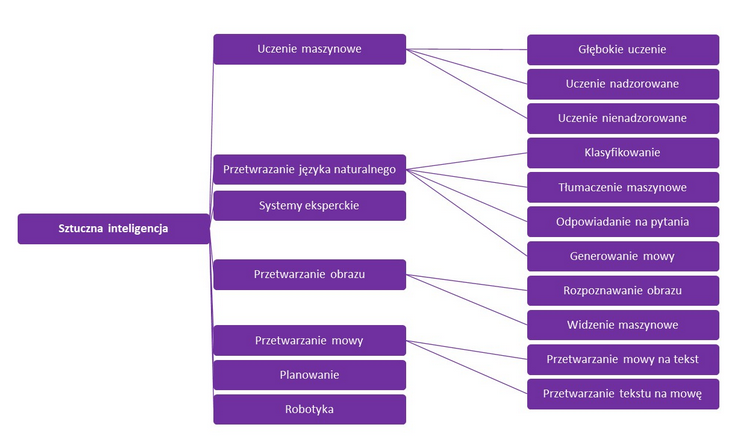
\includegraphics[width=1\linewidth]{AI.png}
    \caption{Obszary zastosowań  sztucznej inteligencji\cite{gov2023}}
\end{figure}

Definicja wg.raportu: "A DEFINITION OF AI:MAIN CAPABILITIES AND DISCIPLINES"  
Sztuczna inteligencja (AI) odnosi się do systemów, które wykazują inteligentne zachowanie poprzez analizę swojego otoczenia i
podejmowanie działań – z pewną dozą autonomii – dla osiągnięcia określonych celów.
Systemy oparte na AI mogą mieć charakter wyłącznie programowy, działać w świecie wirtualnym (np. asystenci głosowi, analiza obrazu
oprogramowanie, wyszukiwarki, systemy rozpoznawania mowy i twarzy) lub sztuczna inteligencja mogą być wbudowane w urządzenia sprzętowe (np.
zaawansowane roboty, samochody autonomiczne, drony czy aplikacje Internetu Rzeczy\cite{ec2029}



\begin{itemize}
    \item \textbf{Uczenie maszynowe (Machine Learning):} Jest to jedna z najważniejszych gałęzi sztucznej inteligencji, która pozwala komputerom na naukę z danych i podejmowanie decyzji na podstawie tych informacji. W ramach uczenia maszynowego wykorzystuje się różne techniki, w tym algorytmy uczenia nadzorowanego i nienadzorowanego.
    
    \item \textbf{Przetwarzanie języka naturalnego (Natural Language Processing - NLP):} Ta dziedzina zajmuje się rozumieniem, przetwarzaniem i generowaniem języka naturalnego przez komputery. NLP jest używane do analizy tekstu, tłumaczenia maszynowego i wielu innych zastosowań.
    
    \item \textbf{Wizja komputerowa:} Obejmuje technologie pozwalające komputerom analizować, rozumieć i interpretować obrazy i wideo. Jest używana w rozpoznawaniu obiektów, rozpoznawaniu twarzy, samochodach autonomicznych i innych dziedzinach.
    
    \item \textbf{Robotyka:} SI jest również istotna w dziedzinie robotyki, gdzie komputery sterują działaniami fizycznymi robotów.
\end{itemize}

\subsubsection{Maszynowe Uczenie}

Maszynowe uczenie (ML) to podzbiór sztucznej inteligencji, który koncentruje się na rozwijaniu algorytmów i technik pozwalających komputerom na naukę z danych i podejmowanie decyzji na podstawie tych informacji. Głównym celem maszynowego uczenia jest rozwijanie modeli, które mogą generalizować zbiory danych i wykonywać zadania bez konieczności programowania ich wprost.

\subsubsection{Zastosowania Maszynowego Uczenia}

Maszynowe uczenie ma szerokie spektrum zastosowań w różnych dziedzinach. W kontekście zarządzania łańcuchem dostaw (SCM), ma to szczególne znaczenie. Poniżej przedstawiamy niektóre z głównych zastosowań ML w SCM:

\begin{itemize}
    \item \textbf{Prognozowanie popytu:} Uczenie maszynowe może być wykorzystywane do prognozowania przyszłego popytu na produkty lub usługi, co pomaga w planowaniu produkcji i zarządzaniu zapasami.
    
    \item \textbf{Optymalizacja zapasów:} Algorytmy ML mogą pomóc w zoptymalizowaniu poziomu zapasów, minimalizując koszty i zapewniając, że dostępność produktów jest na odpowiednim poziomie.
    
    \item \textbf{Wybór dostawcy:} ML może pomóc w analizie dostawców pod kątem efektywności, jakości i kosztów, co ułatwia wybór najlepszego dostawcy.
    
    \item \textbf{Planowanie tras i logistyka:} Algorytmy ML mogą pomóc w optymalizacji tras dostaw, minimalizując czas i koszty transportu.
\end{itemize}

\subsubsection{Rodzaje Maszynowego Uczenia}

Maszynowe uczenie może być podzielone na kilka głównych rodzajów, zależnie od sposobu przetwarzania danych i celu uczenia. Oto niektóre z najważniejszych rodzajów maszynowego uczenia:

\begin{itemize}
    \item \textbf{Uczenie nadzorowane (Supervised Learning):} W tym rodzaju uczenia algorytm jest trenowany na podstawie zestawu danych, który zawiera zarówno wejścia, jak i odpowiadające im oczekiwane wyjścia. Celem jest zbudowanie modelu, który może dokładnie przewidywać wyjście na podstawie nowych danych wejściowych. Przykłady obejmują algorytmy regresji liniowej i klasyfikacji.

    \item \textbf{Uczenie nienadzorowane (Unsupervised Learning):} W przypadku uczenia nienadzorowanego algorytm jest trenowany na danych wejściowych bez oczekiwanych wyjść. Celem jest odkrywanie ukrytych wzorców, grupowanie danych lub redukcja wymiarowości. Przykładem jest klastrowanie danych.

    \item \textbf{Uczenie ze wzmocnieniem (Reinforcement Learning):} Ten rodzaj uczenia polega na trenowaniu agenta, który podejmuje decyzje w środowisku w celu maksymalizacji nagrody. Agent eksploruje różne działania i dostaje informacje zwrotną w postaci nagród lub kar za swoje decyzje. Jest używany w dziedzinach takich jak gry komputerowe i robotyka.

    \item \textbf{Uczenie pół-nadzorowane (Semi-supervised Learning):} Uczenie pół-nadzorowane łączy elementy uczenia nadzorowanego i nienadzorowanego. Model jest trenowany na części danych z etykietami i części danych bez etykiet. Jest stosowane, gdy dostępne są tylko częściowo oznaczone dane.

    \item \textbf{Uczenie głębokie (Deep Learning):} To rodzaj maszynowego uczenia opartego na sieciach neuronowych o wielu warstwach. Jest stosowane do złożonych problemów przetwarzania obrazów, dźwięku i tekstu. Deep Learning osiągnął ogromny sukces w dziedzinach takich jak rozpoznawanie obrazów i przetwarzanie języka naturalnego.

\end{itemize}

Wybór odpowiedniego rodzaju maszynowego uczenia zależy od konkretnego problemu i dostępnych danych. W kontekście zarządzania łańcuchem dostaw, różne rodzaje uczenia maszynowego mogą być stosowane w zależności od konkretnych zadań, takich jak prognozowanie popytu czy optymalizacja tras dostaw.



\subsection{Uczenie maszynowe w zarządzaniu łańcuchem dostaw}
W tym rozdziale dokładniej analizujemy, w jaki sposób maszynowe uczenie może być wykorzystane w zarządzaniu łańcuchem dostaw. Przedstawiamy przykłady konkretnych zastosowań uczenia maszynowego w SCM, takie jak prognozowanie popytu, optymalizacja zapasów czy wybór dostawcy. Omawiamy również korzyści wynikające z wykorzystania tych technik oraz wyzwania, jakie mogą się pojawić.
\subsubsection{Prognozowanie popytu}
Jednym z kluczowych elementów zarządzania łańcuchem dostaw jest zdolność do dokładnego prognozowania popytu na produkty. Maszynowe uczenie oferuje zaawansowane metody analizy danych historycznych oraz czynników wpływających na popyt, co umożliwia dokładniejsze prognozowanie przyszłego zapotrzebowania. Metody te obejmują:

    • Modele szeregów czasowych: Wykorzystują dane historyczne do identyfikowania wzorców w sezonowości i trendach, co pozwala na prognozowanie przyszłego popytu na podstawie danych z przeszłości.
    
    • Algorytmy uczenia maszynowego, takie jak sieci neuronowe i drzewa decyzyjne: Mogą analizować bardziej skomplikowane wzorce w danych, uwzględniając różnorodne zmienne i interakcje między nimi.
    
    • Analiza sentymentu i danych społecznościowych: Wykorzystuje opinię klientów i informacje pochodzące z mediów społecznościowych do oceny wpływu opinii publicznej na popyt na produkty.
    
Precyzyjne prognozy popytu pozwalają firmom lepiej zarządzać swoimi zapasami, minimalizować ryzyko nadmiernego lub niewystarczającego stanu magazynowego oraz dostosować produkcję do rzeczywistych potrzeb rynku.

\paragraph{Modele szeregów czasowych}


Szereg czasowy to ciąg uporządkowanych obserwacji, których dokonuje się w określonych (zwykle stałych) jednostkach czasu. Szeregiem czasowym będzie na przykład średnia cena energii elektrycznej w poszczególnych miesiącach lub ilość zgłaszanych przypadków przemocy domowej w poszczególnych latach. Szereg czasowy można przedstawić w formie wykresu lub tabeli.
Wyróżniamy dwa podstawowe składniki szeregu czasowego – trend i sezonowość. Pojęcie trendu odnosi się do długotrwałej i systematycznej zmiany wielkości danego zjawiska, natomiast sezonowości do rytmicznych, powtarzających się zmian wielkości danego zjawiska, charakteryzujące się różną długością całego cyklu. 
Celem analizy szeregów czasowych jest identyfikowanie i analiza jego struktury, jak również prognozowanie – przewidywanie wartości w kolejnych odstępach czasu, np. sprzedazy. Istnieje wiele metod analizy szeregów czasowych, z czego wiele z nich jest złożonych i obejmują one m.in. analizę trendu (techniki wygładzania) i sezonowości (badanie struktury autokorelacji), modelowanie i prognozowanie szeregów czasowych (m.in. metody ARIMA, wyrównywanie wykładnicze, analiza harmoniczna, analiza widma).\cite{szereg2023}

Szereg czasowy jest bardzo często wykreślany za pomocą wykresu przebiegu (który jest wykresem liniowym czasowym). Szeregi czasowe są wykorzystywane w statystyce, przetwarzaniu sygnałów, rozpoznawaniu wzorców, ekonometrii, finansach matematycznych, prognozowaniu pogody, przewidywaniu trzęsień ziemi,inżynierii sterowania, astronomii, inżynierii komunikacji i głównie w każdej dziedzinie nauk stosowanych i inżynierii, która obejmuje pomiary czasowe.Analiza szeregów czasowych obejmuje metody analizy danych szeregów czasowych w celu wyodrębnienia znaczących statystyk i innych cech charakterystycznych danych. Prognozowanie szeregów czasowych polega na wykorzystaniu modelu do przewidywania przyszłych wartości na podstawie wcześniej zaobserwowanych wartości. Chociaż analizę regresji często wykorzystuje się w celu sprawdzenia zależności między jednym lub większą liczbą różnych szeregów czasowych.W kontekście statystyki, ekonometrii, finansów ilościowych, sejsmologii, meteorologii i geofizyki głównym celem analizy szeregów czasowych jest prognozowanie. W kontekście przetwarzania sygnałów, inżynierii sterowania i inżynierii komunikacji służy do wykrywania sygnału. Inne zastosowania obejmują eksplorację danych, rozpoznawanie wzorców i uczenie maszynowe, gdzie analizę szeregów czasowych można wykorzystać do grupowania, (uwaga od artykulu zrodla!!)klasyfikacji,  zapytań według treści,  wykrywania anomalii i prognozowania.\cite{series2023}
\newpage
Poniżej znajdują się elementy szeregu czasowego:

- Sezonowość: Ten element jest powiązany z kalendarzem,  stałe lub okresowe wachania szeregu czasowego zmiennego w czasie,  istnieje a powtarzający się wzór.

- Trend: Ten komponent odnosi się do długoterminowego trendu wartości obserwacji które z czasem mogą się zwiększać lub zmniejszać.

- Cykliczny: Ten składnik odnosi się również do okresowych wachań czasu serii, ale w odróżnieniu od składnika sezonowości nie jest on stały 

- Losowy: Po wyodrębnieniu wszystkich trzech pozostałych składników z czasu w serii pozostaje element losowy, zwykle ma on strukturę, którą należy zidentyfikować za pomocą modelu w celu dokładnego prognozowania przyszłej wartośi szeregu czasowego.
\cite{Shekh2018}


Mozna wyróżnic wiele modeli szeregów czasowych stosowane do prognozowania :

\begin{figure}[h!]
    \label{fig:S1}
    \centering 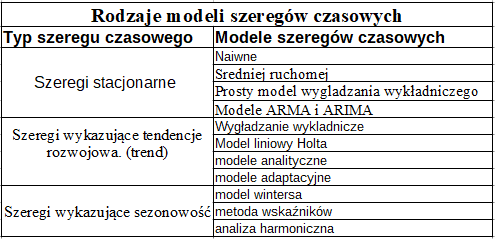
\includegraphics[width=0.5\linewidth]{s1a.png}
    \caption{s1a Modele szeregów czasowych\cite{szer2009}}
\end{figure}

Modele szeregów stacjonarnych. Stacjonarność oznacza, że statystyczne właściwości szeregu czasowego, takie jak średnia i wariancja, są stałe w czasie lub nie zmieniają się w sposób istotny.  Modele stacjonarne zakładają, że szereg czasowy ma ustalone właściwości, co ułatwia analizę i prognozowanie. Istnieje kilka popularnych modeli szeregów stacjonarnych, w tym: 

Model ARMA (AutoRegressive Moving Average): Model ten łączy dwie podstawowe komponenty - autoregresję (AR), która uwzględnia zależności między obserwacjami w czasie, oraz średnią ruchomą (MA), która uwzględnia wpływ losowych zakłóceń. 

Autoregresja to jest model stacjonarny ktory do predykcji przyszlych wartosci uzywa: stalej + przeszlych danych (np jak w modelu AR moze byc 2 rzedu wowczas 2 ostatnich pomiarow) + współczynnika autoregresji  na podstawie danych historycznych , im wyzszy tym ostatnie dane maja wiekszy wplyw na wynik + współczynnik błedu \cite{auto2023}\cite{autor2023}



\(Yt = C + \Theta \cdot Y{t-1} + Et\)

Model autoregresji\cite{mod2023}


To znaczy, zgodnie z modelem AR (1), zmienna y w czasie t jest równa stałej (c), plus zmienna w (t-1) pomnożona przez współczynnik plus błąd. Należy zauważyć, że stała „c” może być liczbą dodatnią, ujemną lub zerową.Jeśli chodzi o wartość teta, czyli współczynnik pomnożony przez y (t-1), może przyjmować różne wartości.

MODEL ARIMA, czyli AutoRegressive Integrated Moving Average, to bardziej zaawansowany model szeregów czasowych, który łączy w sobie trzy główne składniki: model autoregresji (AR), model średniej ruchomej (MA) i różnicowanie (I, od ang. Integrated).  Jest modelem powstalym na bazie ARMA. W przypadku braku różnicowania model przeksztalca sie w ARMA.\cite{Musz2012}\cite{Farz2020}


 Metoda naiwna – metoda prognostyczna dotycząca analizy szeregów czasowych bez tendencji.Metoda ta stosowana jest przy stałym poziomie zjawiska i niewielkich wahaniach przypadkowych
Zalety: 

    • prosta i łatwa do zrozumienia 
    
    • szybka i tania

Wady:

    • niska jakość prognoz 
    
    Jest to prognoza typu: "jutro będzie tak jak dziś"
 \cite{naiw2023}\cite{Shekh2018} 

Mogą być stosowane w przypadku stwierdzenia niewielkich wachań w szeregu zmiennej prognozowanej i wykorzystane w prognozowaniu krótkookresowym, obejmującym jeden okres naprzód. 
Metody naiwne są szybkie i tanie w zastosowaniu, jednak jakość prognoz wyznaczonych z ich użyciem jest zwykle niska.
Przykłady:sprzedaż przedsiębiorstwa w następnym  kwartale będzie na dotychczasowym poziomie,
zysk wzrośnie w tym samym stopniu co ubiegłym miesiącu.\cite{szer2009}

Metoda naiwna, algorytm prognozowania

Y*t = Yt-1

gdzie Y*t prognoza zmiennej Y dla momentu t, Yt-1 to obserwacja rzeczywistej wartosci zmiennej Y dla chwili t-1,Metoda naiwna\cite{szer2009}



Metoda sredniej ruchomej:  Polega na zastępowaniu danych empirycznych dla kolejnych okresów średnimi poziomami z okresu badanego i kilku okresów sąsiednich. Metoda średniej ruchomej może być stosowana zarówno do wygładzania szeregu czasowego, jak i do prognozowania.

\(Y_t = \frac{1}{k} \sum_{i=t-k}^{t-1} Y_i\)

gdzie Yt to prognoza zmiennej Y dla momentu t, Yt obserwacja rzeczywistej wartości zmiennej Y dla chwili i, k to liczba ruchomych skladników szeregu czasowego

srednia ruchoma algorytm\cite{szer2009}



Zalety: prosty algorytm, szybkie i tanie prognozowanie

Wady:koniecznosc doboru stalej K (min. ilosci błedów) dla duzego K potrzeba trzymania duzej ilości danych
Dla usprawnienia dzialania mozna dodac czynnik wag do algorytmu to znaczy ze okres maja rozną wartośc (troche komplikuje algorytm).
Jest to prognoza krótkookresowa, typowa stacjonarna  gdzie zakladamy ze prognozowany okres bedzie podobny ostatnich k - okresów\cite{szer2009}






Model wykladzania wykładniczego.
Wygładzanie wykładnicze (ang. exponential smoothing) – metoda obróbki szeregu czasowego zmniejszająca jego wariancję za pomocą ważonej średniej ruchomej z przeszłych wartości, o wagach malejących wykładniczo wraz z odległością w czasie. Stosowana do prostego usuwania szumu(Stosunek sygnału do szumu (SNR, ang. signal-to-noise ratio) – miara porównująca poziom sygnału użytecznego (informacja) do poziomu szumu tła (niepożądany sygnał). Jest definiowana jako stosunek mocy sygnału użytecznego do mocy szumu tła i jest często wyrażona w decybelach (dB). ) . Jest przydatna w prognozowaniu szeregów czasowych o niewielkim stosunku sygnału do szumu, szczególnie niemających wyraźnego trendu i wahań sezonowych. \cite{wyg2023}

Jest rozszerzeniem idei średniej ruchomej i polega na:wygładzeniu oryginalnego szeregu tak, jak robi to średnia ruchoma ,użycia otrzymanego szeregu do uzyskania przyszłych wartości 
zmiennej, Istotne jest zwiększenie wpływu ostatnich wartości szeregu na 
prognozę, w stosunku do wpływu bardziej odległych obserwacji ,Największa waga jest nadana bieżącej obserwacji, mniejsza waga poprzedniej obserwacji i tak dalej. Wagi zmniejszają się 
geometrycznie w miarę cofania się w czasie. Jest to prosty i szybki algorytm typowy do danych stacjonarnych i nadaje sie na krotkookresowe prognozy\cite{szer2009}
\begin{align*}
Y'_t & = \alpha \cdot Y_{t-1} + (1 - \alpha) \cdot Y'_{t-1} \\
& = Y'_{t-1} + \alpha \cdot (Y_{t-1} - Y'_{t-1})
\end{align*}
gdzie  Y't to prognoza zmiennej Y dla momentu t, Yt-1 to obserwacja rzeczywtistej wartosci zmiennej Y dla chwili t-1, \(\alpha\) to parametr usrdniania (wygładzania) z przedzialu [0,1]


 Wygładzanie wykładnicze algorytm\cite{szer2009}







Kolejna grupa metod to wlączajace w prognoze trend naleza do nich:  metoda liniowa Holta, modele analityczne i adaptacyjne


\vspace{\baselineskip}
Model Holta stosujemy wygładzając szereg czasowy, w którym wyróżnić można zarówno trend (tendencję rozwojową) jak i wcahania przypadkowe.  występuja dwa parametry: alfa i beta.\cite{hol2023}
 \vspace{\baselineskip}
Model Holta pozwala na wygładzanie szeregu czasowego, w którym występuje tendencja rozwojowa oraz wachania przypadkowe. Wartości prognozowanego szeregu zostały oznaczone symbolami x0, x1, ..., xn-1. Model ten ma dwa parametry alfa oraz beta i następującą postać:

\begin{align*}
F_t & = \alpha\cdot X_t + (1 - \alpha)\cdot (F_{t-1} + S_{t-1}) \\
S_t & = \beta\cdot (F_t - F_{t-1}) + (1 - \beta)\cdot S_{t-1}
\end{align*}

gdzie t= 2,...,n-1,

Ft - wygładzona wartość szeregu czasowego,

St - wygldzona wartość przyrostu trendu na moment t,

\(\alpha \beta\) - parametry modelu

Model Holta  obliczanie składnikow szeregu czasowego i trendu\cite{szos2012}





Parametry modelu Holta alfa oraz beta są dobierane tak, aby zminimalizować błędy prognoz\cite{szos2012}

Podwójne wygładzanie wykładnicze –Metoda HOLTA Przystosowane do szeregów czasowych ze składnikami 
sezonowymi i trendami.  Ogólna idea polega na tym, że prognozy są obliczane nie tylko 
na podstawie kolejnych poprzednich obserwacji (jak w prostym  wyrównywaniu wykładniczym), ale można także dodać niezależny trend i składnik sezonowy. 
 Wiele empirycznych szeregów czasowych zawiera wachania sezonowe. (np. roczna sprzedaż komputerów osiąga prawdopodobnie szczyt w listopadzie i grudniu i być może latem) Wzorzec ten będzie się prawdopodobnie powtarzał co roku, chociaż względna wielkość wzrostu sprzedaży w grudniu może się powoli zmieniać z roku na rok.Metoda nadaje sie do krotkookresowej prognozy. Zalety elastycznosc zas  wady trudnosc doboru parametrow\cite{szer2009}





algorytm prognozowania:\\
równanie 1 (usrednienie szeregu czasowego)\\
\begin{align*}
F_{t-1} & = \alpha \cdot Y_{t-1} + (1 - \alpha) \cdot (F_{t-1} + S_{t-1}) \\
\end{align*}
równanie 2 (usrednianie trendu)\\
\begin{align*}
S_t & = \beta \cdot (F_t - F_{t-1}) + (1 - \beta) \cdot S_{t-1} \\
\end{align*}
równanie 3 (wyznaczenie prognozy):\\
\begin{align*}
Y'_t & = F_n + (T - n) \cdot S_n
\end{align*}

gdzie Ft-1 to usredniona prognoza zmiennej Y dla chwili t-1, St-1 to usredniony trend zmiany wartości zmiennej Y dla chwili t-1, \(\alpha  \beta\) to parametry usredniania z przedziału [0,1], Y't to prognoza zmiennej Y dla chwili t, b to liczba elementów szeregu czasowego

Model Holta  cały algorytm\cite{szer2009}


Kolejny przyklad: Potrójne wygładzanie wykładnicze Metoda Wintersa

Model Holta-Wintersa działa na zasadzie „wygładzania” danych szeregów czasowych za pomocą trzech równań wygładzania: dla poziomu, trendu i sezonowości. W efekcie model jest w stanie uwzględnić zmiany zarówno w trendzie, jak i w sezonowości, dostarczając dokładniejsze prognozy.\cite{exc2018}
Model Wintersa może być stosowany w przypadku szeregów czasowych zawierających tendencję rozwojową, wahania sezonowe oraz wahania przypadkowe. \cite{win2023}





\begin{align*}
L_{t-1} & = \alpha \cdot \frac{Y_{t-1}}{C_{t-1-r}} + (1 - \alpha) \cdot (L_{t-2} + B_{t-2}) \\
B_{t-1} & = \beta \cdot (F_{t-1} - F_{t-2}) + (1 - \beta) \cdot B_{t-2} \\
S_{t-1} & = \gamma \cdot \frac{Y_{t-1}}{F_{t-1}} + (1 - \gamma) \cdot S_{t-1} - r
\end{align*}

gdzie:

Lt-1 odpowiednik wygladzonej wartosci otrzymanej z prostego modelu wygladzania wykladniczego (ocena wartosci średniej)

Bt-1 ocena przyrostu trendu na moment lub okres t-1

St-1 ocena wskaźnika sezonowościna moment lub okres t-1

r długość cyklu sezonowego 

a,b i c  parametru modelu przyjmujące wartości z przedziału [0,1]

Model Wintersa  obliczane składniki \cite{win2023}

   \vspace{\baselineskip} 

pelny algorytm:


Potrójne wygładzanie wykladnicze 

Metoda Wintersa
\begin{align*}
F_t & = \alpha \cdot (Y_t - S_{t-r}) + (1 - \alpha) \cdot (F_{t-1} + T_{t-1}) \\
T_t & = \beta \cdot (F_t - F_{t-1}) + (1 - \beta) \cdot T_{t-1} \\
S_t & = \gamma \cdot (Y_t - F_t) + (1 - \gamma) \cdot S_{t-r}  \\
Y'_t & = F_n + (\tau - n) \cdot T_n + S_{t-1} \\
\tau > n
\end{align*}
Ft wygładzona wartość zmiennej prognozowanej

Tt= St wygładzona wartośc przyrostu trendu

St=Ct ocena wskaźnika sezonowosci na momement t

alfa  stała wygladzania poziomu zmiennej F

beta  stała wygładzania współczynnika trendy T

gama stała wygladzania efektu sezonowego S

r długość cykli sezonowości

n numer ostatniej obserwacji

Model Wintersa  pelny algorytm \cite{szer2009}




\newpage

\paragraph{Algorytmy uczenia maszynowego}


 w maszynowym uczeniu mozna wyodrebnic:
 
Uczenie nadzorowane (ang. supervised learning) – sposób uczenia, w którym zbiór danych treningowych, na których uczy się algorytm, zawiera dołączone rozwiązanie problemu, tzw. etykiety albo klasy. 

Uczenie nienadzorowane(ang. unsupervised learning) – sposób uczenia modelu, w którym dane uczące są nieoznakowane tzn. nie posiadają etykiet. Mówiąc potocznie, posiadamy surowe dane które wrzucamy do modelu i zostawiamy algorytmowi całą pracę wiązaną ze znalezieniem powiązań między danymi (tzw. uczenie bez nauczyciela).

Uczenie przez wzmacnianie(ang. RL - reinforcement learning) – jeden z trzech głównych nurtów uczenia maszynowego, którego zadaniem jest interakcja ze środowiskiem na podstawie zebranych informacji. W przeciwieństwie do wymienionych wcześniej rodzajów, w uczeniu przez wzmacnianie nie przygotowuje się zestawu danych uczących, tylko środowisko, z którego model będzie zbierał dane automatycznie. 

  Uczenie półnadzorowane(ang. semisupervised learning) – algorytmy działające na częściowo oznakowanych danych\cite{gove2023}

 Algorytmy prognozowania ML często wykorzystują techniki obejmujące bardziej złożone cechy i metody predykcyjne, ale cel metod prognozowania ML jest taki sam, jak w przypadku metod tradycyjnych – poprawa dokładności prognoz przy jednoczesnej minimalizacji funkcji straty. Funkcję straty przyjmuje się zwykle jako sumę kwadratów spowodowaną błędami w przewidywaniu/prognozowaniu. Najważniejsza różnica pomiędzy obiema metodami polega na sposobie minimalizacji. Chociaż większość tradycyjnych metod wykorzystuje wyjaśnialne procesy liniowe, większość metod ML wykorzystuje techniki nieliniowe w celu minimalizacji funkcji strat. 



Oto kilka przykładów modeli prognozowania uczenia maszynowego stosowanych w aplikacjach biznesowych:

    • Artificial neural network
    
    • Long short-term-memory-based neural network
    
    • Random forest
    
    • Generalized regression neural networks
    
    • K-nearest neighbors regression
    
    • Classification and regression trees (CART)
    
    • Support vector regression
    
    • Gaussian processes 
\cite{gen2023}


w literaturze poswieconej stosowaniu maszynowego uczenia w prognozowaniu popytu spotkalem sie ze najczesciej stosowane modele do prognozowania popytu to:

Neural Networks (NN), zwane również sztucznymi sieciami neuronowymi, są inspiracją biologicznych neuronów. Składają się z warstw neuronów (lub węzłów), które przetwarzają dane i przekazują informacje między sobą za pomocą wag.

Recurrent Neural Networks (RNN) to rodzaj sieci neuronowych, które posiadają pętle rekurencyjne, które pozwalają im na uwzględnianie informacji z poprzednich kroków czasowych w analizie sekwencji danych..

Support Vector Machines (SVM) to technika uczenia maszynowego stosowana zarówno do zadań klasyfikacji, jak i regresji.Tutaj jest wybierana hiperpłaszczyzna decyzyjna które najlepiej oddziela klasy i pozwala prognozowac (na podstawie danych treningowych i cech), optymalizuje margines (miedzy najblizszymi punktami danych a hiperplaszczyzna- wektory nosne), uzywa funkcje jadrowe ktore umowzliwaja przeksztalcanie danych do wyzszych wymiarow/przestszeni gdzie zostaja liniowo odseparowane (mimo ze zaleznosci nie sa liniowe). Najbardziej popularne to :  RBF (Radial Basis Function) i funkcja wielomianowa. Dobierane sa parametry np bledu ktore powoduja zwiekszenia lub zmniejszenie czulosci na dokladnosc( czasami warto dopuscic pewna ilosc bledow niektore dane sa 'wyjatkami')

dodatkowo  KNN (K najbliższych sąsiadów)  jeden z algorytmów regresji nieparametrycznej używanych w statystyce do prognozowania wartości pewnej zmiennej losowej. Może również być używany do klasyfikacji. k-NN może być używane do prognozowania popytu poprzez identyfikowanie podobnych wzorców historycznego popytu do obecnej sytuacji.używamy dane historyczne dotyczących popytu jako zestawu treningowego. Każdy punkt danych reprezentuje przeszły wzorzec popytu i zawiera cechy takie jak pora roku, promocje,  itp. Gdy chcesz prognozować przyszły popyt, obliczasz podobieństwo (odległość) między obecną sytuacją a k-najbliższymi historycznymi wzorcami popytu.

Drzewo decyzyjne,jest intuicyjnym narzędziem do prognozowania, które pozwala na interpretację wyników i jest często używane w analizie danych i uczeniu maszynowym. są często stosowane w prognozowaniu popytu, aby uwzględnić hierarchiczną strukturę czynników wpływających na popyt.
Jak to działa: Buduje drzewo decyzyjne na podstawie danych historycznych, gdzie popyt jest zmienną docelową, a różne czynniki (np. cena, wydatki , sezonowość) są cechami wejściowymi. Drzewo jest budowane poprzez rekurencyjne dzielenie danych na podzbiory na podstawie najważniejszej cechy, aż zostaną spełnione kryteria zatrzymania.

Modele ML dziela dane na zbiór uczacy i testowy, dla kazdego z nich bardzo wazna jest jakosc danych ktore sie wprowadza, odpowiednie oznaczanie cech, żaden z nich nie bedzie dobrze dzialal jest zostana wprowadzone do uczenia dane złej jakości. Dobór danych do uczenia ma bezposredni wpływ na dzialanie kazdego agorytmu ML.

Np. SVM bardzo dobrze radzi z wieloma czynnikami.Zdolność do radzenia sobie z danymi o wielu wymiarach: SVM są skuteczne w przekształcaniu danych do przestrzeni o wysokiej liczbie wymiarów.Efektywnie radzi sobie z danymi nieliniowymi: SVM mają wbudowaną zdolność do radzenia sobie z danymi nieliniowymi, dzięki zastosowaniu funkcji jądrowych, które pozwalają na transformację danych do przestrzeni o wyższej wymiarowości, gdzie mogą być liniowo separowalne.
RNN i NN jak i SVM dobrze radza sobie ze skomplikowanymi danymi, nieliniowymi zaleznosciami. Nieliniowość jest jednym z kluczowych atutów modeli maszynowego uczenia nad tradycyjnymi modelami opartymi o szeregi czasowe.Oto dlaczego nieliniowość jest główną zaletą tych modeli:Zdolność do modelowania skomplikowanych zależności: W rzeczywistych problemach, zależności między danymi często są skomplikowane i nieliniowe.Zdolność do rozwiązywania problemów klasyfikacji nieliniowej: W zadaniach klasyfikacji, gdzie celem jest podział danych na różne klasy, istnieją sytuacje, w których granica decyzyjna między klasami nie jest liniowa.Zdolność do wydobywania nieliniowych wzorców w danych: W przypadku analizy danych, często istnieją nieliniowe wzorce lub zależności, które mogą być trudne do wykrycia za pomocą tradycyjnych modeli liniowych. Elastyczność w dostosowywaniu się do danych: Modele nieliniowe pozwalają na bardziej elastyczne dopasowanie do różnych rodzajów danych

Wsteczna propagacja błędu w czasie, pozwala na uczenie się wzorców na dowolnej głębokości
w szeregu czasowym. Sama wstepna propagacja pomaga na biezaco dopasowywac model: Wsteczna propagacja błędu w czasie (ang. Backpropagation Through Time, BPTT) to technika uczenia sieci RNN poprzez dostosowywanie wag na podstawie błędów prognoz w kolejnych krokach czasowych. Pozwala to na aktualizację wag w sieci, aby minimalizować błąd prognozowany przez model.

Dodatkowo tradycyjne metody czesto maja blad tzw. efekt bata . Efekt "bata" (ang. "bullwhip effect") jest zjawiskiem występującym w łańcuchu dostaw i zarządzaniu zapasami, które polega na zwiększającej się zmienności i niestabilności zamówień w miarę przesuwania się w górę łańcucha dostaw od ostatecznego punktu sprzedaży do dostawcy surowców. To zjawisko może prowadzić do nadmiernego wzrostu kosztów i nadmiar zapasów, co jest niekorzystne dla efektywności łańcucha dostaw i rentowności firmy.
Główne przyczyny efektu "bata" obejmują:

-Nadmierną zmienność zamówień: Zamówienia przekazywane przez kolejne ogniwa łańcucha dostaw mogą być podatne na oscylacje, gdzie zamówienia na jednym etapie mogą znacznie różnić się od rzeczywistego popytu na końcu łańcucha dostaw.

-Opóźnienia w komunikacji: Informacje o rzeczywistym popycie i zamówieniach mogą być przekazywane z opóźnieniem między różnymi uczestnikami łańcucha dostaw, co powoduje nieaktualne i niestabilne prognozy.

-Zwiększanie zamówień bez odpowiedniej przyczyny: W odpowiedzi na niestabilność i oscylacje w zamówieniach, uczestnicy łańcucha dostaw mogą zwiększać zamówienia, aby zabezpieczyć się przed niedoborami, co dalej pogarsza efekt "bata".

Z efektem 'bata' ML radzi sobie znacznie lepiej od tradycyjnych metod poniewaz:

-Modele ML, takie jak SVM, RNN i ANN, mają zdolność do wykrywania bardziej skomplikowanych wzorców w danych i uwzględniania nieliniowych zależności. Mogą bardziej precyzyjnie modelować zmiany w popycie.

-Lepsza adaptacja do danych czasowych: Modele sa przydatne do prognozowania danych czasowych, takich jak historia zamówień, ponieważ uwzględniają sezonowość i zmienne warunki

-Automatyczna adaptacja: Modele ML mogą być trenowane i dostosowywane do zmieniających się warunków rynkowych i danych, co pozwala na lepsze dostosowanie się do dynamicznych sytuacji.

-Integracja z danymi w czasie rzeczywistym: Modele ML mogą być dostosowywane do analizy danych w czasie rzeczywistym, co pozwala na reakcję na zmiany w czasie rzeczywistym.


Dodatkowym waznym aspektem jest aspektem jest w jakiej prognozie krótko czy długoterminowej widac bardziej zalety uczenia maszynowego. Zdecydowanie w krótkoterminowym. Krótkoterminowe prognozy (na kilka dni, tygodni lub kilka miesięcy).Uczenie maszynowe (ML) może być bardziej przydatne w krótkoterminowych prognozach, gdy mamy do czynienia z nieliniowymi zależnościami i dynamicznymi zmianami w danych. Modele ML mogą lepiej radzić sobie z przewidywaniem krótkoterminowych fluktuacji popytu, które mogą być wynikiem sezonowości, trendów rynkowych lub innych skomplikowanych czynników. Długoterminowym okresie zmiany sa bardziej przewidywalne i czesciej mozna uzywac tradycyjnych metod związanych z szeregami czasowymi.Tradycyjne metody mogą nadal być skuteczne w długoterminowych prognozach, zwłaszcza w przypadku stabilnych czynników wpływających na popyt. 
Niemniej gdy przychodzi do dlugoterminowej prognozy i podjecia decyzji jaka metode uzyc to wg. Katherine Gail Nowadly  and Sohyun Jung z Massachusets Institue of Technology najczesciej stosowane sa SVM, ANN\cite{Gail2020}

\cite{carb2006}\cite{Mary2022}\cite{wikknn2023}\cite{Shekh2018}\cite{Xiao2021}\cite{Resul2017}\cite{Farz2020}\cite{Carbo2007}\cite{Shahr2009}\cite{Gail2020}




Dla oceny jakosci prognozy popytu  czesto stosuje sie MAPE i RMSE.
MAPE (Mean Absolute Percentage Error) to popularna metryka używana do oceny jakości prognoz w problemach prognozowania popytu lub innych zadań regresji. MAPE pozwala na ocenę dokładności prognoz w sposób procentowy, co jest szczególnie przydatne do porównywania prognoz między różnymi zestawami danych lub modelami.


\begin{align*}
& \left( \frac{1}{n} \sum_{i=1}^{n} \frac{|aktualny_i - prognozowany_i|}{|aktualny_i|} \right) \cdot 100
\end{align*}

MAPE \cite{Shekh2018}


RMSE to skrót od "Root Mean Square Error", co w tłumaczeniu na język polski oznacza "Pierwiastek błędu średniokwadratowego". Jest to miara błędu, która jest często używana w statystyce i analizie danych do oceny dokładności modelu lub prognoz w stosunku do rzeczywistych danych.

Róznica miedzy nimi jest w 'kwadracie' potegowanie w RMSE skutkuje ze jest bardzej wrazliwy na duze błedy niz MAPE.



wyrażenie matematyczne dla RMSE wyglada nastepująco:

\begin{align*}
\text{RMSE} &= \sqrt{\frac{1}{n} \sum_{i=1}^{n} (Y_i - \hat{Y}_i)^2}
\end{align*}

n to liczba punktów danych w zestawie testowym

Yi to rzeczywista wartość w i-tym punkcie danych

\(\hat{Y}_i\) to wartość prognozowana przez model w i-tym punkcie danych



\newpage
\subsubsection{Optymalizacja zapasów}

\paragraph{Wprowadzenie}


Optymalizacja zapasów (zarządzanie zapasami) polega na skutecznym zarządzaniu ilościami produktów przechowywanych w magazynach. Głównym celem jest zminimalizowanie kosztów magazynowania, jednocześnie zapewniając wystarczający poziom dostępności produktów, aby zaspokoić popyt klientów. Tradycyjne metody zarządzania zapasami, takie jak metoda ABC czy metoda EOQ (Economic Order Quantity), są stosunkowo statyczne i nie uwzględniają zmienności popytu i innych czynników.
Samo zarządzanie zapasami skupia sie na 4 kwestiach:
Koncentruje się na czterech zasadniczych kwestiach:

   - ile jednostek należy zamówić (lub wyprodukować) w danym czasie,
   
   - kiedy należy złożyć zamówienie,
   
  -  które składniki zapasów wymagają szczególnej uwagi,
  
 -   czy można zabezpieczyć się przed wzrostem kosztów zapasów.
 \vspace{\baselineskip} 
  Głowne metody stosowane to:
  
 - Reguła 80/20 - na jej bazie została stworzona metodyka ABC, dzieli zapasy pod kątem wartości. Skoro 20 procent pozycji stanowi 80procent całkowitej wartości zapasu, to sugeruje odmienne podejście do sterowania zapasem tych 20procent pozycji, do procesu wyboru dostawców oraz do obsługi dostaw.

 - Metoda ABC polegająca na podziale zapasów na trzy grupy. Podział ten oparty jest na założeniu, że zapasy, które ilościowo stanowią duży udział w zapasach ogółem, lecz mały pod względem wartościowym. I odwrotnie: są też takie zapasy, których udział wartościowy jest duży, a mały ilościowo. Dzieli materiały (lub wytwarzane produkty) na ważne, mniej ważne i nieważne. 
 
-Metoda XYZ(metoda ilościowa) jest uzupełnieniem metody ABC, w której zapasy rozpatruje się z punktu widzenia regularności zapotrzebowania i dokładności prognozowania. Klasa X zawiera asortymenty, na które występuje regularne zapotrzebowanie (popyt). Klasa Y stanowi asortyment, na który występują sezonowe wahania w zapotrzebowaniu. Klasa Z składa się z asortymentu, na który występuje sporadyczne (okazjonalne) zapotrzebowanie. 

-Model ekonomicznej (optymalnej) wielkości zamówienia - EOQ (Economic Order Quantity) jest najbardziej rozpowszechnioną koncepcją wykorzystywaną w zarządzaniu zapasami materiałów i towarów. Wraz ze wzrostem wielkości zamówienia wzrasta poziom przeciętnych zapasów, a to z kolei powoduje spadek kosztów tworzenia i wzrost kosztów utrzymania zapasów. Jeżeli natomiast częstotliwość zamówień się zwiększy, to wielkość przeciętnych zapasów spadnie, zmniejszą się także koszty utrzymania, a wzrosną koszty tworzenia zapasów. 

-Metoda "dokładnie na czas" (just- in- time JIT) polega na tym że, system gospodarki zapasami, w którym niezbędne materiały wpływają dokładnie wtedy, kiedy są potrzebne, bez zakłóceń procesu produkcji, co pomaga organizacji kontrolować zapasy surowców, ograniczając zapotrzebowanie na powierzchnię magazynową. System ten zmniejsza zakres niezbędnych nakładów organizacji na przestrzeń magazynową potrzebna do przechowywania materiałów i na same materiały. Polega ona na również na zamawianiu materiałów i części, w mniejszych partiach, zmniejszając tym samym nakłady na przestrzeń magazynową oraz nakłady zamrożone w samych zapasach. 


Koszty zapasow mozemy podzielic na 3 czesci:


   - koszty tworzenia zapasów(ang. Ordering Costs):

    Są to koszty związane z procesem zamawiania i tworzenia nowych zapasów. Obejmuje to koszty związane z przygotowywaniem zamówień(koszty procesów informacyjnych), kontrolowaniem poziomu zapasów, negocjacjami z dostawcami(Koszty informacyjne ), kosztami przewozu, a także kosztami związanymi z ewentualnym przyjęciem i magazynowaniem nowych dostaw.
  
   
   - koszty utrzymania zapasów,

   To koszty związane z przechowywaniem i utrzymaniem zapasów w magazynie lub na innych powierzchniach przechowalniczych.Składają się z następujących elementów: koszty kapitałowe: inwestycje w zapasy, koszty magazynowania: magazyny fabryczne, magazyny publiczne, magazyny dzierżawne, magazyny własne, koszty obsługi zapasów: ubezpieczenie, podatki,koszty ryzyka: utrata wartości, uszkodzenia, ubytki, koszty zmiany lokalizacji.
    
  -koszty niedoboru zapasów.

  koszty przestojów produkcyjnych, To koszty związane z brakiem zapasów w momencie, gdy są one potrzebne ,koszty utraconej sprzedaży mogą obejmować straty z tytułu utraty klientów, spadku sprzedaży oraz koszty utraconej reputacji a także ewentualne koszty pilnych zamówień lub dostaw w celu zaspokojenia brakujących zapasów.. 
 
 
\cite{enc2023}\cite{Prav2020}\cite{Hanne2017}


\paragraph{Wykorzystanie uczenia maszynowego w optymalizacji zapasów}

'stare' metody sa statyczne nie uwzgledniaja zmian, opieraja sie na max kilku cechach (zazwyczaj 2 cechy: cena, zapotrzebowanie) jakiekolwiek zmiany wymagaja duzej pracy ludzkiej, nie dostosowuja sie do zmian, nie sa elastyczne, nie radza sobie z duza iloscia danych, . ML ten sam algorytm moze pracowac zarowno dla malej jak i duzej firmy dla kazdego produktu, pod produktu, polproduktu jak i rodzin produktowych (tam gdzie armia ludzi w biurze i magazynie jest potrzebna do obslugi uzywajac tradycyjnych metod). Tradycyjne metody były wykorzystywane przez kilkadziesiat lat ale mozliwosci jakie daje maszynowe uczenie pozwala na usprawnienie pracy

Maszynowe Uczenie oferuje:

Dopasowanie do zmiennego popytu: W przeciwieństwie do tradycyjnych metod, które zakładają stałe lub statystyczne wartości (np. stałą wielkość zamówienia w EOQ), algorytmy uczenia maszynowego są w stanie dostosowywać się do zmiennej natury popytu. Mogą analizować historyczne dane sprzedaży i innych czynników wpływających na popyt, co pozwala na generowanie dokładniejszych prognoz

Real-time reakcje: Uczenie maszynowe pozwala na monitorowanie i dostosowywanie poziomów zapasów w czasie rzeczywistym. Gdy zmieniają się warunki rynkowe, takie jak sezonowość, trendy konsumenckie lub zmiany w dostawach, algorytmy ML mogą reagować szybciej niż statyczne metody.

Automatyzacja zamawiania ,Sztuczna inteligencja zapewnia przewagę w postaci automatycznego ponownego zamawiania, czyli funkcji, która może znacznie poprawić efektywność zapasów. Na podstawie przewidywania trendów sprzedaży i aktualnych poziomów zapasów sztuczna inteligencja może we właściwym czasie uruchamiać automatyczne zamówienia uzupełniające, zapewniając w ten sposób optymalny poziom zapasów.

Analiza wielu czynników: ML może uwzględniać wiele czynników jednocześnie. Oprócz historii sprzedaży może analizować dane meteorologiczne, trendy konsumenckie, promocje , zmiany cen i wiele innych. Dzięki temu może lepiej zrozumieć, co wpływa na popyt i dostosować się do tych zmian.

Zwiększona precyzja: ML może dostarczyć bardziej precyzyjne prognozy popytu, co pomaga w uniknięciu nadmiarowych zapasów (które generują koszty magazynowania) lub braków w dostawach (co wpływa na obsługę klienta i straty finansowe).

Wykrywanie anomalii: Algorytmy uczenia maszynowego są również zdolne do wykrywania anomalii w danych magazynowych, co pozwala na szybkie reagowanie na nieprawidłowości w poziomach zapasów.

Personalizacja: ML może dostosowywać strategie zarządzania zapasami do konkretnych rodzajów produktów, co pozwala na bardziej efektywne podejście w zależności od charakterystyki produktów.
\cite{linn2023}\cite{cdp2023}\cite{Matti2023}\cite{Had2023}

W literaturze spotykam ponizsze algorytmy maszynowego uczenia stosowane do optymalizacji zapasów:
SVM, SVR, RNN, ANN, drzewa decyzyjne, Q-Learning. wiekszosc z nich została juz skrótowo opisana w poprzednim podrozdziale. Tutaj na uwage zasługuje jeszcze nie opisywany SVR i Q-Learning

SVR (Support Vector Regression) to algorytm uczenia maszynowego wykorzystywany do rozwiązywania problemów regresji, czyli przewidywania wartości numerycznych na podstawie danych treningowych. Działa on na podobnej zasadzie co SVM (Support Vector Machine) w przypadku klasyfikacji, ale jest dostosowany do problemów regresji zas SWM klasyfikuje dane i je dzieli.Regresja to pojęcie w statystyce i analizie danych, które odnosi się do procesu modelowania zależności między jedną lub wieloma zmiennymi niezależnymi (czynnikami) a zmienną zależną (wartością, którą chcemy przewidzieć). Głównym celem regresji jest znalezienie matematycznego modelu lub funkcji, która opisuje, jak zmienne niezależne wpływają na zmienną zależną.

Q-Learning to algorytm uczenia maszynowego, który jest często wykorzystywany do uczenia się optymalnych strategii w problemach decyzyjnych z uczeniem ze wzmocnieniem.Ogólna idea Q-Learning polega na uczeniu agenta, jakie akcje podejmować w danej sytuacji, aby maksymalizować sumę nagród na przestrzeni wielu kroków czasowych. Algorytm ten jest często używany w kontekście gier i problemów, w których agent interaktywnie działa w pewnym środowisku.Oto główne kroki algorytmu Q-Learning: 

-Inicjalizacja tabeli Q: Tworzona jest tabela (lub macierz) Q, która przechowuje wartości Q dla wszystkich dostępnych stanów i akcji.

- Wybór akcji: Agent rozpoczyna w pewnym stanie środowiska. Na podstawie wartości Q wybierana jest akcja, którą agent chce podjąć. Może to być akcja wybrana w sposób zachłanny (na podstawie maksymalnej wartości Q) 

- Wykonanie akcji: Agent wykonuje wybraną akcję i przechodzi do nowego stanu środowiska.

-Obserwacja nagrody i nowego stanu: Agent obserwuje, ile nagrody otrzymuje za podjętą akcję oraz jaki jest nowy stan środowiska, do którego przeszedł.

-Aktualizacja wartości Q: Wartość Q dla danej pary stanu i akcji jest aktualizowana na podstawie otrzymanej nagrody i przewidywanej przyszłej wartości Q. Istnieje wiele czynników, które sprawiają, że Q-learning ma kluczowe znaczenie:

Dlaczego używamy q-learning? Po pierwsze, bez wyraźnego programowania komputery mogą uczyć się na nowych ustawieniach i dostosowywać się do nich. Nazywa się to Q-learningiem. Należałoby napisać wyraźne instrukcje dla każdej istotnej okoliczności, z jaką może spotkać się komputer w tradycyjnym programowaniu. Komputer jest bardziej wszechstronny i dostosowuje się do nowych scenariuszy dzięki Q-learningowi, który pozwala mu na samodzielną naukę metodą prób i błędów.
Po drugie, różnorodne procesy decyzyjne, w tym te w robotyce, teorii gier i finansach, można zoptymalizować za pomocą Q-learningu. Q-learning może pomóc komputerom w dokonywaniu bardziej przydatnych ocen w skomplikowanych kontekstach poprzez identyfikację najlepszego sposobu działania lub zbioru działań, które maksymalizują długoterminową nagrodę.

Odnosnie zarzadzania zapasami, q-learning jest wstanie podejmowac decyzje co zamowic ?kiedy? ile? po jakiej cenie? jest wstanie podejmowac optymalne decyzje w srodowisku ktore jest dynamiczne, ma bardzo duzo danych , dzieki permanentnej eksploracji ten model jest wstanie osiagnac znacznie wiecej niz czlowiek z tradycyjnymi modelami. Mozna bez problemu wprowadzic otoczenie dla agenta gdzie bedzie koszt zamawiania, koszt zakupu, koszt trzymania materialu, przychod ze sprzedazy, koszt braku materiału na stanie itp...

\cite{Had2023}\cite{wiksvr2023}\cite{alakh2023}\cite{intell2023}





\newpage
\subsubsection{Planowanie produkcji}
 \vspace{\baselineskip} 
\paragraph{Planowanie produkcji}
 \vspace{\baselineskip} 

to uzgodnienie asortymentu oraz ilości wyrobów gotowych, które są przewidziane do wytworzenia, a także rozłożenie ich produkcji w czasie, tak aby zrealizować plan sprzedaży i osiągnąć zakładany zysk i aby sprostać zapotrzebowaniu rynku. Jest to istotny element zarządzania łańcuchem dostaw oraz efektywnego wykorzystywania zasobów produkcyjnych.
Planowanie dotyczy zarówno aspektów technicznych, jak i organizacyjnych, ekonomicznych i zarządzania. Ważne parametry to specyfika wyrobów, terminy rozpoczęcia i zakończenia procesu produkcyjnego oraz chronologiczne czynności w procesie wytwarzania. Planowanie produkcji może być na rok, uwzględniając zdolności produkcyjne i zasoby, oraz wsteczne lub do przodu. Główny harmonogram produkcji ma na celu efektywne wykorzystanie zasobów, utrzymanie poziomu obsługi klientów i minimalizację kosztów. Istnieją różne warianty tworzenia harmonogramu, a planowanie produkcji może być międzywydziałowe, wewnątrzwydziałowe lub ogólnozakładowe. Planowanie produkcji może być operacyjne, taktyczne lub strategiczne, zależnie od horyzontu czasowego i hierarchii w procesie planowania. 
Planowanie produkcji obejmuje planowanie procesów, surowców i zasobów w celu wytworzenia towarów dla konsumentów w określonych ramach czasowych. Harmonogram produkcji określa, kto i kiedy będzie przeprowadzał operacje.


Główne cele planowania produkcji to:

1.ciągłość przepływu produkcji – jednym z głównych celów planowania i kontroli produkcji jest ciągły przepływ produkcji przez zakład produkcyjny. Ciągłe doskonalenie przepływu i procesów to jedna z integralnych koncepcji Lean Manufacturing, Six Sigma i ogólnego usprawnienia produkcji. Planowanie i kontrola produkcji będzie próbą osiągnięcia płynnego i ciągłego procesu produkcyjnego poprzez wyeliminowanie wąskich gardeł i marnotrastwa z zakładu, co pozwoli  przenieść produkcję na wyższy poziom pod względem produktywności.

2.Planowane zasobów — element planowania produkcji i kontroli produkcji jest niezbędny, aby mieć pewność, że  zakład produkcyjny ma to, czego potrzebuje, we właściwej ilości i we właściwym czasie. Posiadanie planu produkcji gwarantuje, że masz wystarczającą ilość materiałów, maszyn, narzędzi, sprzętu i siły roboczej do wykonania pracy.


3.Optymalny poziom zapasów — zapasy są często uważane za marnotrawstwo w operacjach produkcyjnych. Dzieje się tak dlatego, że koszty związane z zapasami stanowią jedne z największych kosztów ponoszonych w przypadku wielu operacji. Dlatego też należy dążyć do maksymalnego zmniejszenia poziomu zapasów, aby odpowiednio obniżyć koszty w swojej działalności. Planowanie i kontrola produkcji planuje oraz realizuje procesy, które umożliwiają spójny przepływ produkcji, aby ostatecznie zbliżyć się do produkcji JIT (dokładnie na czas) i zmniejszyć poziom zapasów w operacjach produkcyjnych.

4.Zwiększona produktywność – zwiększona produktywność to kolejny istotny cel w ramach planowania i kontroli produkcji. Planowanie i kontrola produkcji ostatecznie ma na celu zwiększenie produktywności poprzez poprawę wydajności, a jednocześnie jest ekonomiczne. Zwiększoną produktywność udaje się osiągnąć poprzez optymalizację wykorzystania istniejących zasobów produkcyjnych i zasobów pracy, przy jednoczesnej eliminacji marnotrawstwa/psucia materiałów.

5.Zadowolenie klienta - Wszystkie firmy chcą zwiększać zadowolenie klientów. Dzieje się tak dlatego, że popyt jest napędzany przez klientów, a zadowoleni klienci oznaczają więcej transakcji w przyszłości. Posiadanie wadliwych produktów i opóźnienia w dniach wysyłki będą tylko szkodliwe dla firmy. Planowanie i kontrola produkcji koncentruje się przede wszystkim na zapewnieniu, że proces produkcyjny skutecznie i terminowo realizuje zamówienia oraz skróceniu czasu realizacji. Dzięki temu zamówienia klientów zostaną zrealizowane terminowo i w krótkim czasie, co wpłynie na poprawę zadowolenia klientów z Twojej firmy.





Podziały planowania produkcji:

    1. Planowanie strategiczne produkcji: To długoterminowe planowanie, które obejmuje okres od kilku lat do kilkunastu lat. Służy osiągnięciu celów strategicznych oraz zrealizowaniu misji przedsiębiorstwa. Powinno uwzględniać zmiany w otoczeniu rynkowym. Jego podstawą są prognozy ekonomiczne, badania marketingowe, a także zapotrzebowanie na wyrób , ustala ogólne kierunki rozwoju produkcji i dostosowanie jej do strategii przedsiębiorstwa. W tym rodzaju planowania uwzględnia się m.in. inwestycje w nowe zakłady produkcyjne, rozwijanie nowych produktów i technologii.
    
    2. Planowanie taktyczne produkcji: To planowanie na średni okres czasu, zazwyczaj obejmuje okres od kilku miesięcy do kilku lat. Obejmuje przygotowanie produkcji (m.in. plan zapotrzebowania na niezbędne zasoby, zarządzanie zapasami, utrzymanie maszyn, sterowanie jakością wyrobów), marketing, dystrybucję wyrobów, badanie i rozwój wyrobu oraz plany przepływów środków finansowych. Celem jest dostosowanie produkcji do zmieniającego się popytu, zachowując przy tym odpowiedni poziom zasobów i elastyczność w produkcji. W ramach tego planowania tworzy się tzw. plany produkcyjne, które określają harmonogramy produkcji na podstawie prognoz popytu.
    
    3. Planowanie operacyjne produkcji: To planowanie krótkoterminowe, obejmuje najbliższe dni, tygodnie lub miesiące. Odnosi się do działań jednorazowych, które nazywamy projektami. Najczęściej obejmują przygotowanie produkcji oraz działania powtarzalne, które dotyczą procesów wytwarzania wyrobów. Celem jest precyzyjne ustalenie harmonogramu produkcji na podstawie aktualnych danych o stanie magazynów, dostawach surowców i aktualnym popycie. W ramach tego planowania tworzy się tzw. harmonogramy produkcyjne, które określają, co i kiedy ma być produkowane.
    
    4. Planowanie reaktywne: To rodzaj planowania, które występuje w przypadku nieoczekiwanych zakłóceń w procesie produkcji, takich jak awarie maszyn, opóźnienia dostaw, czy zmiany w zamówieniach klientów. Celem jest szybka reakcja na te zakłócenia i minimalizacja negatywnych skutków dla produkcji.

    Podział planowania produkcji ze względu na typ produkcji:

    1. Planowanie oparte na zadaniu ,jednostkowa (custom-made)

Produkcja oparta na zadaniu lub projekcie koncentruje się na wytwarzaniu pojedynczego produktu i jest obsługiwana przez jednego pracownika lub grupę osób (każdy produkt jest wykonywany na zamówienie klienta, zazwyczaj w pojedynczych egzemplarzach lub w niewielkich seriach), w przypadku zadań na małą skalę, które wymagają bardzo mało specjalistycznego sprzętu, jest stosunkowo łatwe do wykonania. Rodzaje zadań objętych tego typu planowaniem produkcji mogą dotyczyć małej skali, np. tworzenia biżuterii na zamówienie. Większe, bardziej złożone projekty produkcyjne, takie jak budowa domów na zamówienie, również należą do tej kategorii.Pozwala to na wykonanie produktów według życzeń klienta i zazwyczaj może zostać włączone w dowolnym momencie procesu produkcyjnego, nie zakłócając jego przebiegu.Planowanie produkcji jednostkowej jest bardzo elastyczne i opiera się na dostosowaniu do indywidualnych potrzeb klienta. Procesy produkcyjne są unikalne dla każdego produktu.


2.Produkcja seryjna (batch production)

Produkcja seryjna ma zastosowanie, gdy elementy są produkowane w grupach, a nie indywidualnie lub w ramach produkcji ciągłej. Produkty są wytwarzane w partiach lub seriach o stałej wielkości. Na przykład ciastka są produkowane partiami, co oznacza, że każdy etap produkcji w danej partii ciastek odbywa się w tym samym czasie. Zaczyna sie od odmierzania składników całej porcji, następnie zmieszasz je ze sobą, a na koniec upieczesz je razem, tak aby cały proces produkcji partii ciasteczek rozpoczynał się i kończył w tym samym czasie.

Wyzwaniem, , jest uwzględnienie ograniczeń na każdym etapie operacji, aby zapewnić maksymalizację wydajności zasobów bez przekraczania maksymalnego dozwolonego limitu. Na przykład, jeśli Twój mikser do ciasta zmieści partię 100 ciastek, ale możesz upiec tylko 300 na raz, możesz napotkać wąskie gardła w produkcji.

Planowanie produkcji seryjnej ma na celu zoptymalizowanie procesów produkcyjnych dla konkretnej partii, minimalizując zmiany w konfiguracji maszyn i narzędzi.
    
3. Produkcja przepływowej (flow production)

Produkcja przepływowa to metoda sterowana popytem, charakteryzująca się ciągłym przepływem jednostek przez linię produkcyjną.Produkcja przepływowa (flow production) obejmuje procesy produkcyjne, w których produkty są wytwarzane w ciągłym przepływie, bez przerw i z minimalnymi zmianami w konfiguracji maszyn , narzędzi . Ten typ produkcji jest często stosowany w sektorach takich jak przemysł motoryzacyjny, produkcja elektroniki ,przemysł spożywczy lub w produkcji telewizorów i sprzętu AGD, gdzie produkt wytwarzany jest w drodze szeregu zbiorowych operacji, podczas których materiały przechodzą z jednego etapu do drugiego bez opóźnień i przerw.

Kluczowe cechy produkcji przepływowej obejmują:

    Ciągłość produkcji: Procesy produkcyjne działają nieprzerwanie, aby utrzymać stały przepływ produktów przez linię produkcyjną.

    Standaryzacja: Produkty są zazwyczaj standardowe i podlegają minimalnym zmianom w trakcie produkcji.

    Automatyzacja: W produkcji przepływowej stosuje się automatyzację w dużym stopniu, aby zminimalizować udział pracy ręcznej i zwiększyć wydajność.

    Optymalizacja przepływu: Planowanie produkcji przepływowej skupia się na optymalizacji sekwencji operacji produkcyjnych, aby zapewnić płynny przepływ produktów.

    Wysoka wydajność: Produkcja przepływowa ma na celu osiągnięcie jak najwyższej wydajności i minimalizację kosztów jednostkowych.

    
Korzyści płynące z metody przepływowej produkcji polegają na tym, że producenci mogą zminimalizować liczbę produktów w toku i wyrobów gotowych przechowywanych w zapasach, obniżyć koszty i skrócić czas realizacji produkcji.

4.Metoda masowej produkcji

Produkcja masowa jest bardzo podobna do produkcji przepływowej. Technika ta jest bardzo korzystna przy produkcji dużej liczby tych samych przedmiotów w krótkim czasie.Produkty są wytwarzane w dużej skali, zazwyczaj w stałych seriach.

Ten rodzaj produkcji jest zwykle zautomatyzowany, co zmniejsza koszty pracy potrzebnej do produkcji. Niektóre zakłady produkcyjne posiadają linie montażowe dedykowane dla określonego rodzaju przedmiotu, co skraca wymagany czas przezbrajania i zwiększa ogólną wydajność produkcji. Pozwala to producentom zwiększyć zyski, ponieważ koszty produkcji są znacznie obniżone.

Planowanie produkcji masowej ma na celu osiągnięcie maksymalnej wydajności i minimalizację kosztów jednostkowych.

    
 5. Produkcja ciągła lub procesowa(continuous production): W produkcji ciągłej procesy produkcyjne działają przez całą dobę bez przerwy, rodzaj procesu ciągłego podobnego do produkcji masowej i produkcji przepływowej, ale charakteryzuje się ciągłym przepływem materiałów przez linię produkcyjną. Ten typ produkcji jest często stosowany w branżach chemicznej, petrochemicznej i wytwarzania energii. Planowanie produkcji ciągłej ma na celu utrzymanie stałego przepływu produkcji i minimalizację przestojów.
 Zazwyczaj wyroby gotowe wytworzone w tego typu produkcji nie są liczone jako odrębne jednostki. Na przykład produkcja i przetwarzanie cieczy, gazów lub chemikaliów, gdy produkt jest wytwarzany w jednolitej i znormalizowanej kolejności.

Metoda Procesowa wykorzystuje specyficzne i wyrafinowane maszyny do przetwarzania materiałów na każdym etapie operacji. W tego typu produkcji nie ma miejsca na błędy, ponieważ zmiana jednego typu przedmiotu na inny będzie wymagała długiego okresu przezbrojenia. Często w wyniku tego rodzaju produkcji powstają produkty uboczne lub odpady.

    
6. Produkcja w linii montażowej (assembly line production): Ten typ produkcji opiera się na przemieszczaniu produktu przez linię montażową, gdzie każdy etap montażu jest wykonywany przez innego pracownika lub maszynę. Planowanie produkcji w linii montażowej ma na celu zoptymalizowanie sekwencji i czasu wykonywania poszczególnych operacji.
    
7. Produkcja projektowa (project production): W produkcji projektowej każdy produkt lub projekt jest unikalny, a procesy produkcyjne są dostosowywane do konkretnych projektów. Planowanie produkcji projektowej wymaga skomplikowanej koordynacji zasobów i harmonogramowania działań.
    

Podział ten wynika z różnic w rodzaju produktów, ilościach produkowanych jednostek, rodzaju procesów produkcyjnych i elastyczności produkcji. Planowanie produkcji musi być dostosowane do specyficznych wymagań każdego typu produkcji, aby osiągnąć efektywność i spełnić oczekiwania klientów.


Istnieje wiele innych odmian planowania produkcji, które koncentrują się na różnych aspektach procesu produkcyjnego. Oto kilka z nich:

 A.  Główny harmonogram produkcji (Master production schedule MPS)

Są to harmonogramy produkcji dla określonych towarów, które muszą być produkowane oddzielnie. Często są tworzone przez oprogramowanie, a następnie modyfikowane przez użytkowników.Plan ten określa ilościowo istotne procesy, części i inne zasoby w celu optymalizacji produkcji, identyfikacji wąskich gardeł oraz przewidywania potrzeb i gotowych towarów. Ponieważ MPS napędza dużą działalność fabryki, jego dokładność  dramatycznie wpływają na rentowność. Typowe MPS są tworzone przez oprogramowanie z możliwością modyfikacji przez użytkownika.
 Zwykle jest to powiązane z produkcją, gdzie plan wskazuje, kiedy i ile będzie zapotrzebowanie na każdy produkt. Plan ten określa ilościowo istotne procesy, części i inne zasoby w celu optymalizacji produkcji, identyfikacji wąskich gardeł oraz przewidywania potrzeb i gotowych towarów.harmonogramy nie obejmują wszystkich aspektów produkcji, a jedynie kluczowe elementy, które udowodniły swoją skuteczność kontrolną, takie jak prognozowany popyt, koszty produkcji, koszty zapasów, czas realizacji zamówienia, godziny pracy, wydajność, poziom zapasów, dostępne miejsce do przechowywania i dostawę części. Wybór tego, co modelować, różni się w zależności od firmy i fabryki.MPS przekłada zapotrzebowanie klientów (zamówienia sprzedaży) na plan budowy, wykorzystując zaplanowane zamówienia w prawdziwym środowisku planowania komponentów. Korzystanie z MPS pomaga uniknąć niedoborów, kosztownych przyspieszeń, planowania w ostatniej chwili i nieefektywnej alokacji zasobów.
 Jak działa mps?. Wykorzystując wiele zmiennych jako dane wejściowe, MPS wygeneruje zestaw wyników wykorzystywanych do podejmowania decyzji. Dane wejściowe mogą obejmować prognozowany popyt, koszty produkcji, wartośc zapasów, potrzeby klientów, dostawy , wielkość partii, czas realizacji produkcji i wydajność. Dane wejściowe mogą być automatycznie generowane przez system ERP łączący dział sprzedaży z działem produkcji.Wyniki mogą obejmować ilości, które mają zostać wyprodukowane, poziom zatrudnienia, dostępną ilość do obiecania i przewidywane dostępne saldo. Wyniki można wykorzystać do stworzenia harmonogramu planowania wymagań materiałowych (MRP).

 Efektywny MPS :
 
Zapewni produkcji, planowaniu, zakupom i zarządzaniu informacje umożliwiające planowanie i kontrolowanie produkcji. Powiąże ogólne planowanie biznesowe i prognozowanie ze szczegółowymi operacjami.Umożliwi marketingowi podejmowanie uzasadnionych zobowiązań w zakresie dostaw do magazynów i klientów. Zwiększy wydajność i dokładność produkcji w firmie zapewni zgrubne planowanie wydajności.

B.Planowanie zapotrzebowania materiałowego (MRP)

MRP to system zarządzania zapasami, harmonogramowania i planowania produkcji. Dostępność surowców gwarantuje system MRP, który utrzymuje również wewnętrzne poziomy materiałów i produktów na możliwie najniższym poziomie.

Planowanie wymagań materiałowych (MRP) to system planowania, harmonogramowania i kontroli zapasów, używany do zarządzania procesami produkcyjnymi. Większość systemów MRP opiera się na oprogramowaniu.
System MRP ma jednocześnie spełniać trzy cele:

     - Upewnij się, że surowce są dostępne do produkcji, a produkty są dostępne do dostawy do klientów.
     
    - Utrzymuj najniższy możliwy poziom materiałów i produktów 
    
     -Planuje działania produkcyjne, harmonogramy dostaw i działania zakupowe.

 Do podstawowych funkcji systemu MRP zalicza się: kontrolę zapasów, przetwarzanie list materiałowych i elementarne planowanie.  Służy do planowania działań związanych z produkcją, zakupami i dostawami.MRP jest narzędziem pozwalającym uporać się z tymi problemami. Zawiera odpowiedzi na kilka pytań: Jakie elementy są wymagane?Ile jest potrzebnych? Kiedy są potrzebne?...    
 Dane, które należy wziąć pod uwagę, obejmują:

     Tworzony element końcowy . Nazywa się to czasem niezależnym popytem lub poziomem „0” na BOM (bill of material zestawieniu materiałów).
     
     Ile potrzeba teraz.
     
     Kiedy ilości są wymagane, aby zaspokoić popyt.
     
     Okres trwałości przechowywanych materiałów.
     
     Stan zapasów. Ewidencja materiałów netto dostępnych do wykorzystania już w magazynie (od ręki) oraz materiałów na zamówienie u dostawców.
     
     Zestawienia materiałów. Szczegóły dotyczące materiałów, komponentów i podzespołów wymaganych do wytworzenia każdego produktu.
     
     Dane planistyczne. Obejmuje to wszystkie ograniczenia i wskazówki dotyczące produkcji takich przedmiotów, jak: trasa, standardy pracy i maszyn, standardy jakości i testowania, polecenia pull/work cell i push, techniki ustalania wielkości partii (tj. stała wielkość partii, partia za partią), procent złomowania i inne dane wejściowe.

     dane wyjsciowe:

     Wyjścia

Istnieją dwa wyjścia i różne komunikaty/raporty:

     Wynik 1 to „Zalecany harmonogram produkcji”. Określa szczegółowy harmonogram wymaganych dat rozpoczęcia i zakończenia, wraz z ilościami dla każdego etapu wyznaczania trasy i zestawienia materiałów wymaganych do zaspokojenia zapotrzebowania z głównego harmonogramu produkcji (MPS).
     
     Wynik 2 to „Zalecany harmonogram zakupów”. Określa to zarówno daty, w których zakupione artykuły powinny zostać przyjęte do zakładu, jak i daty, w których powinny nastąpić zamówienia zakupu lub wydanie zamówienia zbiorczego, aby dopasować się do harmonogramów produkcji.


     C.Planowanie zdolnosci produkcyjnych (capacity planning)

Jest to proces sprawdzania, jak dobrze firma jest przygotowana do radzenia sobie ze zmieniającymi się wymaganiami.to proces określania zdolności produkcyjnej potrzebnej organizacji, aby sprostać zmieniającemu się zapotrzebowaniu na jej produkty. W kontekście planowania wydajności zdolność projektowa to maksymalna ilość pracy, jaką organizacja lub osoba jest w stanie wykonać w danym okresie. Rozbieżność między możliwościami organizacji a wymaganiami jej klientów skutkuje nieefektywnością wynikającą z niedostatecznego wykorzystania zasobów lub niespełnionego zapotrzebowania klientów. Celem planowania zdolnościprodukcyjnych jest zminimalizowanie tej rozbieżności. Zapotrzebowanie na zdolność organizacji zmienia się w zależności od zmian w wielkości produkcji, takich jak zwiększanie lub zmniejszanie wielkości produkcji istniejącego produktu lub wytwarzanie nowych produktów. Lepsze wykorzystanie istniejącej wydajności można osiągnąć poprzez poprawę ogólnej efektywności sprzętu (OEE). 

 szerokie klasy planowania zdlonosci produkcyjnych obejmują strategię wiodącą, strategię opóźnień, strategię dopasowania i strategię dostosowania:

 -  Wiodącą strategią jest zwiększanie wydajności zgodnie z rosnącym popytem. Strategia wiodąca to strategia agresywna, której celem jest odciągnięcie klientów od konkurentów firmy poprzez poprawę poziomu usług i skrócenie czasu realizacji. To także strategia mająca na celu redukcję kosztów braków magazynowyc

 -    Strategia opóźnienia odnosi się do dodawania mocy produkcyjnych dopiero wtedy, gdy organizacja pracuje z pełną wydajnością lub przekracza ją ze względu na wzrost popytu . Jest to strategia bardziej konserwatywna i przeciwna strategii wiodącej wydajności. Zmniejsza to ryzyko marnotrawstwa, ale może skutkować utratą potencjalnych klientów w wyniku wyczerpania zapasów lub niskiego poziomu usług

 -Strategia dopasowania polega na zwiększaniu wydajności w małych ilościach w odpowiedzi na zmieniający się popyt na rynku. Jest to bardziej umiarkowana strategia.

 D.Planowanie produkcji poziomowane(level production planning)

 to rodzaj planowania produkcji, który koncentruje się na wytwarzaniu stałej wielkości produkcji w danym okresie. Oznacza to, że przez cały okres produkcji wykorzystywana jest ta sama ilość surowców i zasobów, co zapewnia stałą i przewidywalną produkcję.

Celem tego rodzaju planowania jest osiągnięcie wysokiej efektywności i redukcja kosztów poprzez zapewnienie możliwie najbardziej efektywnego wykorzystania zasobów.

E.Planowanie odchudzone (lean production planning)

Lean Production Planning to rodzaj planowania produkcji, który koncentruje się na minimalizacji odpadów i optymalizacji wykorzystania zasobów. Ten rodzaj planowania kładzie nacisk na stosowanie małych partii i eliminację nadprodukcji. Celem odchudzonego planowania produkcji jest redukcja kosztów, zwiększenie wydajności i poprawa zadowolenia klientów.

F. Planowanie produkcji Kaizen

Planowanie produkcji Kaizen to rodzaj planowania produkcji, który koncentruje się na ciągłym doskonaleniu i optymalizacji procesów. Ten typ planowania kładzie nacisk na wykorzystanie danych i informacji zwrotnych w celu zidentyfikowania obszarów wymagających poprawy i wprowadzenia zmian, które zwiększą wydajność i obniżą koszty.

G Zwinne planowanie produkcji (agile planning)

Zwinne planowanie produkcji to rodzaj planowania produkcji, który koncentruje się na podejmowaniu szybkich i skutecznych decyzji. Ten rodzaj planowania kładzie nacisk na wykorzystanie danych i informacji zwrotnych w celu szybkiego podejmowania decyzji i szybkiego dostosowywania się do zmieniających się warunków.



sam proces planowania produkcji wyglada nastepujaco:

Opis procesu
1. Zdobycie informacji na temat zapotrzebowania (ile , jaki towar, kiedy i gdzie jest potrzebny)

2. Zdobycie informacji na temat stanów magazynowych(ile , jaki towar,  gdzie jest )


3. Analiza pracochłonności i materiałochłonności
oszacowanie materiałochłonności i pracochłonności określonych procesów produkcji. 

4. Złożenie zamówienia na materiały i określenie potrzeb kadrowych

5. Hierarchizacja zleceń
Efektem tej pracy jest informacja o kolejności realizacji zleceń.

6. Określenie przewidywanego czasu realizacji zamówienia
 Efektem pracy jest ustalenie planowych terminów realizacji zleceń

 
7. Sporządzenie szczegółowego planu produkcji

 Efektem całej pracy jest końcowa uszczegółowiona postać planu produkcji
 
8. Aktualizacja bieżącego planu

9. Kontrola i monitorowanie produkcji

10. Informowanie o przebiegu procesu kierowników zaopatrzenia, sprzedaży

 
\cite{encp2023}\cite{pl2023}\cite{pla2023}\cite{des2023}\cite{wikm2023}\cite{wikmr2023}\cite{wikc2023}\cite{Hanne2017}


\newpage
\paragraph{Wykorzystanie uczenia maszynowego w planowaniu produkcji}
 \vspace{\baselineskip} 

 Planowanie produkcji operuje w srodowisku dynamicznym , zmiennym i bardzo zlożonym.Zawsze są odstępstwa pomiędzy planowaniem produkcji i późniejsza realizacja. Te odchylenia wynikają z niepewności, np. niedokładne lub niewystarczające dane dotyczące planowania (np. jakość danych i
dostępność), niewłaściwe systemy planowania i kontroli lub nieprzewidywalne zdarzenia.Dlatego planiści produkcji korzystają z buforów w postaci zapasów . Bufory jednak prowadzą do
zwiększonego wysiłku w zakresie koordynacji i kontroli, zwiększając np.  stan zapasów, czas realizacji . Ponadto stwierdzono, że niezawodność planów produkcyjnych, a tym samym jakość planowania (PQ) może spaść do 25 procent w ciągu pierwszych trzech dni po stworzeniu planu. Maszynowe uczenie wlasnie musi umiec sobie radzic z wymienionymi problemami\cite{ryb2019}

w literaturze fachowej najczesciej spotykane algorytmy/typy maszynowego uczenia stosowanych do planowania produkcji to: Uczenie przez wzmacnianie (Reinforcement Learning, RL) szczegolnie q-learning (jeden z algorytmow uczenia przez wzmocnienie) jak i  siec neuronowa (NN neural networks), spotkalem sie rowniez z uzyciem : regression tree,klastrowanie, drzewo decyzyjne, svm, bootstrap aggregated (bagged) tree, random forest (tutaj jako wsparcie w podejmowaniu decyzji dla poszczególnych elementow planowania), ensable learning (uczenie zespołu ). Ensable learninng  to technika uczenia maszynowego, która łączy kilka podstawowych modeli w celu stworzenia jednego optymalnego modelu predykcyjnego gdzie tworzy sie wiele modeli klasyfikacji lub regresji przy użyciu zbioru danych treningowych Każdy model podstawowy może zostać utworzony przy użyciu różnych podziałów tego samego zestawu danych treningowych i tego samego algorytmu lub przy użyciu tego samego zestawu danych z różnymi algorytmami lub dowolnej innej metody nastepnie podejmowana jest decyzja jaki model wybrac za pomoca głosowania dla klasyfikacji i uśredniania  dla regresji)



Uczenie przez wzmacnianie (Reinforcement Learning, RL) ktore jest dedykowane do niepewnego srodowiska gdzie sa rzeczy znane i nieznane.Środowisko jest zwykle określane w formie procesu decyzyjnego Markowa (MDP Markov Decission Process), ponieważ wiele algorytmów uczenia się przez wzmacnianie w tym kontekście wykorzystuje techniki programowania dynamicznego.
Podstawowe uczenie się przez wzmacnianie jest modelowane jako proces decyzyjny Markowa:
   zbiór stanów środowiska i agenta, S, zbiór działań A agenta,prawdopodobieństwo przejścia (w chwili  t) ze stanu s  do stanu  s' pod działaniem  a,natychmiastowa nagroda po przejściu z s do  s' z działaniem  a.
 

Podsumowujac Uczenie przez wzmacnianie sklada sie z elementow takich jak:
- Agent: Agent to byt uczący się, który podejmuje decyzje w danym środowisku. (moze tworzyc plan produkcji)

- Środowisko: Środowisko to kontekst, w którym agent działa i podejmuje decyzje. Środowisko może być rzeczywiste  lub wirtualne . Środowisko dostarcza informacji zwrotnej w postaci nagród lub kary za działania agenta.To moze być srodowisko produkcyjne

-Akcje: Agent ma zestaw dostępnych akcji, które może podjąć w danym stanie środowiska. Celem agenta jest znalezienie strategii decyzyjnej (polityki), która określa, która akcja powinna być wybrana w odpowiedzi na stan środowiska.NP. moze podejmowac co i kiedy nalezy produkowac

-Stany: Stany opisują aktualny stan środowiska. Mogą to być obserwacje dostępne dla agenta, które zawierają informacje o środowisku w danym momencie.Np moga to byc informacje o dostepnosci materialow, wykonaniu planu produkcji, awarii maszyn itp.

-Nagroda: Nagroda to liczba reprezentująca ocenę jakości działania agenta w danym stanie i po podjęciu danej akcji. Celem agenta jest maksymalizacja sumy nagród w dłuższej perspektywie czasowej.Np mozemy nagradzac za dobry plan produkcji np taki ktory wykorzystal w pelni zdolnosci produkcyjne lub zostal w pelny wykonany (czyli byl realny) zaspokoil zapotrzebowanie klienta itp.

-Polityka: Polityka to strategia decyzyjna agenta, która określa, jakie akcje należy podejmować w odpowiedzi na stany środowiska. Celem uczenia przez wzmacnianie jest znalezienie optymalnej polityki, która maksymalizuje nagrody.NP tu mozna stosowac rozne strategie planistyczne np level planning (rownomierne planowanie produkcji)

w skrócie sam proces wyglada nastepujaco:
 \vspace{\baselineskip}
 
   1. Agent obserwuje aktualny stan środowiska.
   
   2. Na podstawie obserwacji, agent używa swojej strategii decyzyjnej (polityki) do wyboru akcji.
   
  3.  Środowisko wykonuje wybraną akcję i przechodzi do nowego stanu.
  
 4.   Środowisko przekazuje nagrodę za wykonanie akcji.
 
   5.  Agent aktualizuje swoją strategię na podstawie otrzymanej informacji zwrotnej, aby w przyszłości podejmować lepsze decyzje.
   \vspace{\baselineskip} 

   Kilka słow odnosnie procesu decyzyjnego markowa. Jest stochastycznym procesem sterowania w czasie dyskretnym. Zapewnia ramy matematyczne do modelowania podejmowania decyzji w sytuacjach, gdy wyniki są częściowo przypadkowe, a częściowo pod kontrolą decydenta. MDP są przydatne do badania problemów optymalizacyjnych rozwiązywanych za pomocą programowania dynamicznego.Nazwa MDP pochodzi od rosyjskiego matematyka Andrieja Markowa.Proces decyzyjny Markowa to 4-krotka, gdzie: ( S , Z , P  , R  ) S jest zbiorem stanów zwanym przestrzenią stanów,A A to zbiór akcji zwany przestrzenią akcji ,P to prawdopodobieństwo, że działanie A w stanie S w chwili T doprowadzi do stanu S' w chwili t+1,R to natychmiastowa nagroda (lub oczekiwana natychmiastowa nagroda) otrzymana po przejściu ze stanu S do stanu S' w wyniku działania A.
 \vspace{\baselineskip} 
Dlaczego uczenie przez wzmacnianie jest odpowiednie do planowania produkcji?


    1. Dynamiczne i niepewne środowisko: Środowisko produkcyjne często jest dynamiczne i nieprzewidywalne. Procesy produkcyjne mogą być podatne na awarie maszyn, zmienne zapotrzebowanie na produkty, zmiany w dostawach surowców, i wiele innych czynników, które wpływają na efektywność i koszty produkcji. RL pozwala adaptować się do zmieniających się warunków i podejmować decyzje w czasie rzeczywistym.

    2.Optymalizacja celów produkcyjnych: RL może być używane do optymalizacji celów produkcyjnych, takich jak maksymalizacja wydajności, minimalizacja kosztów lub optymalne zarządzanie zapasami. Agent RL może uczyć się optymalnej strategii decyzyjnej, która uwzględnia różne cele i ograniczenia produkcyjne.

    3.Kompleksność problemu: Planowanie produkcji to zazwyczaj zadanie o dużym stopniu trudności, ze względu na wiele zmiennych i ograniczeń. RL pozwala na podejście do tych złożonych problemów i znalezienie rozwiązań w czasie rzeczywistym.


    sa tez uzywane inne algorytmy ktore wspomagaja planiste produkcji ( ale nie wykonuja calej pracy za niego) to wspomniane juz:  Drzewo regresyjne (Regression Tree), Drzewo bagged  (Bagged Tree), Las losowy (Random Forest) lub maszynowe uczenie polaczone z MPC (Model predictive control -model sterowania predykcyjnego). Odnosnie MPC (Model predictive control ) jest to  optymalna technika sterowania, w której obliczone działania sterujące minimalizują funkcję kosztu dla ograniczonego układu dynamicznego w skończonym, oddalającym się horyzoncie.
W każdym kroku czasowym sterownik MPC otrzymuje lub szacuje aktualny stan . Następnie oblicza sekwencję działań kontrolnych, która minimalizuje koszty w horyzoncie czasowym, rozwiązując ograniczony problem optymalizacji.  Modele stosowane w MPC mają generalnie na celu przedstawienie zachowania złożonych i prostych układów dynamicznych. Modele MPC przewidują zmianę zmiennych zależnych modelowanego systemu, która będzie spowodowana zmianami zmiennych niezależnych.
 
    warto wspomniec ze również operacje logistyczne wspierajace planowanie produkcji jak np. obsluga materialow (material handling) która to czynność polegająca na transporcie materiałów w zakładzie produkcyjnym, np. z magazynu do stanowiska pracy, lub ze stanowiska pracy do rampy załadunkowej lub pomiędzy budynkiem a pojazdem . MH  odgrywa znaczącą rolę w
płynnej i terminowej produkcji wyrobów gotowych . Tu równiez istnieje zmienne i  dynamiczne srodowisko i mamy do czynienia ze zlozonym problemem czyli mamy srodowisko ktore pasuje dla RL czyli uczenie przez wzmacnianie. 

\cite{guo2020}\cite{wiku2023}\cite{wikr2023}\cite{wikma2023}\cite{Naw2009}\cite{Faust2019}\cite{gar2020}\cite{gov2021}\cite{ryb2019}\cite{mat2023}\cite{chen2021}\cite{chmiel2019}\cite{Cada2020}\cite{este2023}\cite{ehn2018}




\paragraph{Kolejny poziom podsekcji}

\newpage
\par
\subsection{Kluczowe algorytmy uczenia maszynowego dla łańcucha dostaw}


W tym rozdziale omówimy kluczowe algorytmy uczenia maszynowego, które znajdują zastosowanie w zarządzaniu łańcuchem dostaw. Te algorytmy są wykorzystywane do rozwiązywania różnorodnych problemów związanych z planowaniem, prognozowaniem i optymalizacją w łańcuchach dostaw. Przedstawimy główne algorytmy oraz ich główne zastosowania.

Wśród omawianych algorytmów znajdują się między innymi regresja liniowa, drzewa decyzyjne, sieci neuronowe, maszyny wektorów nośnych oraz algorytmy klastrowania. Dla każdego algorytmu przedstawiamy także przykłady jego potencjalnych zastosowań w SCM.
Celem tych rozdziałów jest zaprezentowanie czytelnikowi podstawowych informacji na temat maszynowego uczenia i jego roli w zarządzaniu łańcuchem dostaw oraz dostarczenie wglądu w kluczowe algorytmy, które mogą być używane do rozwiązywania problemów związanych z SCM.

do tej pory wszystkie wymienione przez mnie modele i algorytmy maszynowego uczenia to:


Uczenie nadzorowane (Supervised Learning):\\
Uczenie nadzorowane polega na szkoleniu modelu za pomocą zbioru treningowego, w którym każda próbka jest opisana etykietą lub odpowiedzią. Celem jest nauczenie modelu przewidywania tych odpowiedzi dla nowych danych. Dwa główne obszary wykorzystujące uczenie nadzorowane to rozwiązywanie problemu regresji (przewidywanie wartości) i problem klasyfikacji (przewidywanie klas). Jako przykład regresji można wskazać prognozowanie wartości samochodu na podstawie jego modelu, marki, roku produkcji, przebiegu, pojemności silnika, rodzaju paliwa itd. Przykładem modelu klasyfikacji jest filtr spamu, czyli problem zakwalifikowania wiadomości jako spam czy nie. \\\\



Przykłady algorytmów uczenia nadzorowanego rozwiązujący problem regresji:\\
    • Support vector regression\\ 
    • Neural Networks (NN)\\
    • Recurrent Neural Networks (RNN)\\
    • K-nearest neighbors regression\\
    • regression tree\\
    •linear regression \\
    •polynomial regression\\
    • Generalized regression neural networks\\
    • Classification and regression trees (CART)\\

    Przykłady algorytmów uczenia nadzorowanego rozwiązujący problem klasyfikacji:\\
    • Support Vector Machines (SVM)\\
    • K-nearest neighbors (KNN)\\
    • naive Bayes classifier\\
    • random forest\\
    •logistic regression \\

Kilka najważniejszych algorytmów z podziałem na problemy, którymi się zajmują:

Analiza skupień:

    metoda k-średnich
    hierarchiczna analiza skupień
    DBSCAN ( density-based spatial clustering of applications with noise)

Wykrywanie anomalii i nowości:

    jednoklasowa maszyna wektorów nośnych

Wizualizacja i redukcja wymiarowości:

    analiza głównych składowych (PCA – ang. principal component analysis)
    jądrowa analiza głównych składowych


    
Uczenie nienadzorowane (Unsupervised Learning):\\
W uczeniu nienadzorowanym nie ma etykiet ani odpowiedzi w zbiorze treningowym. Głównym celem jest odkrywanie struktur lub wzorców w danych. Klastrowanie to przykład, w którym modele grupują dane na podstawie ich podobieństwa, podczas gdy redukcja wymiarowości pomaga zmniejszyć liczbę cech, zachowując istotne informacje. Mówiąc potocznie, posiadamy surowe dane które wrzucamy do modelu i zostawiamy algorytmowi całą pracę wiązaną ze znalezieniem powiązań między danymi (tzw. uczenie bez nauczyciela). Należą do nich m. in. algorytmy analizy skupień (ang. clustering) – inaczej klasteryzacja albo grupowanie. Przykładem problemu analizy skupień jest określenie grup podobnych użytkowników, robiących zakupy w sklepie internetowym albo wchodzących na serwis informacyjny. \\
    • Klastrowanie (Clustering)\\
    • Drzewo decyzyjne (Decision Tree)\\
    • Random forest\\
    • Gaussian processes\\

    
Uczenie ze wzmocnieniem (Reinforcement Learning):\\
 jeden z trzech głównych nurtów uczenia maszynowego, którego zadaniem jest interakcja ze środowiskiem na podstawie zebranych informacji. W przeciwieństwie do wymienionych wcześniej rodzajów, w uczeniu przez wzmacnianie nie przygotowuje się zestawu danych uczących, tylko środowisko, z którego model będzie zbierał dane automatycznie. Jego celem jest zmaksymalizowanie zwracanej przez nie nagrody. Środowisko może być zależne od celu nauki. W przypadku uczenia programu grającego w gry będzie to gra, wraz z jej zasadami, lub prawdziwy świat, w przypadku programu uczącego się sterować łazikiem.\\
W uczeniu przez wzmacnianie wyróżnia się 3 główne elementy:\\

   - Środowisko – to zadanie lub symulacja, z którym algorytm (w tym kontekście nazywany również agentem albo graczem) wchodzi w interakcję. Celem uczenia przez wzmacnianie jest maksymalizacja nagrody zwracanej przez środowisko, czyli nauczenie agenta osiągania w nim najwyższego wyniku, np. wygrania największej ilości gier albo osiągniecia największej stopy zwrotu (jeśli środowisko jest symulacją giełdy).\\
   - Agent – to element, który wchodzi w interakcję ze środowiskiem. Zadaniem agenta jest maksymalizowanie nagrody, czyli nauczenie się najkorzystniejszego oddziaływania ze środowiskiem. Za zachowanie agenta odpowiada tzw. polityka, czyli funkcja, zwracająca akcję. Jako politykę najczęściej stosuje się sieć neuronową.\\
   - Bufor – magazyn danych przechowujący informacje zebrane przez agenta w trakcie uczenia, które są następnie wykorzystane do jego wytrenowania.\\
. \\
przyklad:\\
    • Q-Learning\\\\
Uczenie głębokie (Deep Learning):\\
Uczenie głębokie, często oparte na głębokich sieciach neuronowych, to rodzaj uczenia maszynowego, który jest wysoce zaawansowany i wykorzystywany do rozwiązywania skomplikowanych problemów, takich jak rozpoznawanie obrazów, przetwarzanie języka naturalnego i wiele innych. Modele te składają się z wielu warstw neuronów, które są w stanie automatycznie ekstrahować cechy z danych. \\
    • Neural Networks (NN)\\
    • Recurrent Neural Networks (RNN)\\
\cite{gove2023}

\newpage
\subsubsection{Uczenie nienadzorowane (Unsupervised Learning) }
\paragraph{Klastrowanie}

 Np. grupowanie/klastrowanie (clustering) jest jednym z metod sztucznej inteligencji.Grupowanie, znane również jako klasyfikacja lub analiza skupień, to technika przetwarzania danych wykorzystywana w dziedzinie uczenia maszynowego i sztucznej inteligencji. Polega na dzieleniu zbioru danych na grupy (skupienia) na podstawie podobieństwa między jego elementami. W analizie danych i uczeniu maszynowym termin "clustering" jest szeroko używany i odnosi się do procesu tworzenia grup (klas) obiektów na podstawie pewnych kryteriów, takich jak odległość między obiektami. Celem jest stworzenie skupisk obiektów, które są podobne do siebie wewnątrz klastra, ale różnią się od obiektów w innych klastrach.Istnieje cały szereg algorytmow zastosowan klastrowania w sztucznej inteligencji.

  Klastrowanie to dla uczenia maszynowego nienadzorowanego. Możesz również usłyszeć, że nazywa się to analizą skupień ze względu na sposób działania tej metody.Użycie algorytmu grupowania oznacza, że dasz algorytmowi dużo danych wejściowych bez etykiet i pozwolisz mu znaleźć dowolne grupy w danych, jakie tylko może.Grupy te nazywane są klastrami. Klaster to grupa punktów danych, które są do siebie podobne na podstawie ich relacji do otaczających punktów danych.Kiedy zaczynasz od danych, o których nic nie wiesz, klastrowanie może być dobrym miejscem na uzyskanie wglądu.Istnieją różne typy algorytmów grupowania:
  
 •  Oparte na gęstości.W klastrowaniu opartym na gęstości dane są grupowane według obszarów o dużej koncentracji punktów danych otoczonych obszarami o niskiej koncentracji punktów danych. Zasadniczo algorytm znajduje miejsca gęste z punktami danych i wywołuje te klastry.

 •  Oparta na dystrybucji.W przypadku podejścia klastrowego opartego na dystrybucji wszystkie punkty danych są uważane za części klastra na podstawie prawdopodobieństwa, że należą do danego klastra.Działa to w ten sposób: istnieje punkt środkowy i wraz ze wzrostem odległości punktu danych od środka maleje prawdopodobieństwo, że będzie on częścią tego klastra.

  •  Oparty na centroidach.Jest trochę wrażliwy na parametry początkowe jakie mu podajesz, ale jest szybki i wydajny.Algorytmy tego typu oddzielają punkty danych na podstawie wielu centroidów w danych. Każdy punkt danych jest przypisany do klastra na podstawie kwadratu odległości od środka ciężkości. Jest to najczęściej stosowany rodzaj grupowania.
  
  •  Oparte na hierarchii.Klastrowanie oparte na hierarchii jest zwykle używane w przypadku danych hierarchicznych, takich jakie można uzyskać z firmowej bazy danych lub taksonomii. Buduje drzewo klastrów, dzięki czemu wszystko jest zorganizowane od góry do dołu.\cite{clust2020}

Najbardziej znane algorytmy sztucznej inteligencji bazujaca na klastrowaniu to:
  • Algorytm grupowania K-średnich(K-means).Grupowanie K-średnich jest najczęściej używanym algorytmem grupowania. Jest to algorytm oparty na centroidach i najprostszy algorytm uczenia się bez nadzoru.Algorytm ten próbuje zminimalizować wariancję punktów danych w klastrze. Średnie K najlepiej stosować w przypadku mniejszych zestawów danych, ponieważ iterują po wszystkich punktach danych. Oznacza to, że klasyfikacja punktów danych zajmie więcej czasu, jeśli w zbiorze danych znajduje się ich duża liczba.\cite{clust2020}

Jest to iteracyjny proces przypisywania każdego punktu danych do grup, w wyniku którego punkty danych są powoli grupowane w oparciu o podobne cechy. Celem jest zminimalizowanie sumy odległości między punktami danych a środkiem ciężkości klastra, aby zidentyfikować właściwą grupę, do której powinien należeć każdy punkt danych.Tutaj dzielimy przestrzeń danych na K klastrów i przypisujemy każdemu z nich średnią wartość. Punkty danych są umieszczane w skupieniach najbliższych średniej wartości tego skupienia. Dostępnych jest kilka wskaźników odległości, które można wykorzystać do obliczenia odległośc.
Jak działają K-średnie?
Weźmy przykład, aby zrozumieć, jak krok po kroku działają K-średnie. Algorytm można podzielić na 4-5 kroków.


    A. Wybór liczby klastrów
Pierwszym krokiem jest zdefiniowanie liczby K skupień, w których będziemy grupować dane. Wybierzmy K=3.

    B. Inicjowanie centroidów
Centroid jest środkiem klastra, ale początkowo dokładny środek punktów danych będzie nieznany, dlatego wybieramy losowe punkty danych i definiujemy je jako centroidy dla każdego klastra. Zainicjujemy 3 centroidy w zbiorze danych.

\begin{figure}[h!]
    \label{fig:k1}
    \centering 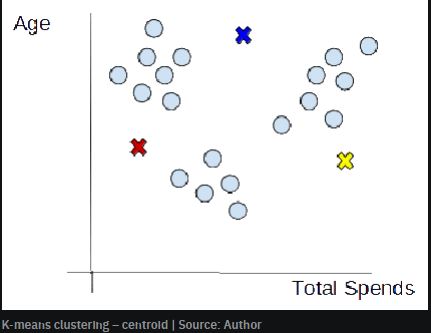
\includegraphics[width=0.8\linewidth]{K1.png}
    \caption{k1 Grupowanie K-średnich\cite{clust2020}}
\end{figure}
 \newpage
 C.Przypisz punkty danych do najbliższego klastra
Teraz, gdy centroidy zostały zainicjowane, następnym krokiem jest przypisanie punktów danych Xn do ich najbliższego środka ciężkości klastra Ck
\begin{figure}[!h]
    \label{fig:k2}
    \centering 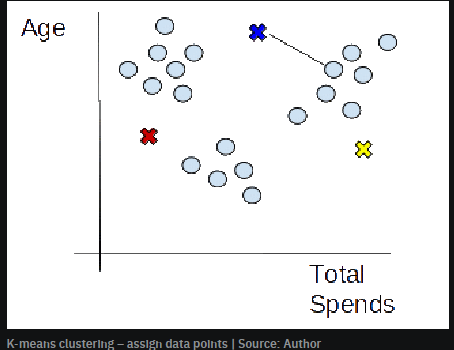
\includegraphics[width=0.8\linewidth]{K2.png}
    \caption{k2 Grupowanie K-średnich przypisanie danych\cite{clust2020}}
\end{figure}

W tym kroku najpierw obliczymy odległość między punktem danych X a środkiem ciężkości C, korzystając z metryki odległości euklidesowej.
Metryka odległości euklidesowej:

\begin{align*}
d(x, y) = \sqrt{\sum_{i=1}^{n} (x_i - y_i)^2}
\end{align*}

Metryka odległości euklidesowej.Wzór\cite{clust2020}


Następnie wybierz klaster dla punktów danych, w których odległość między punktem danych a środkiem ciężkości jest minimalna.
\begin{figure}[h!]
    \label{fig:k4}
    \centering 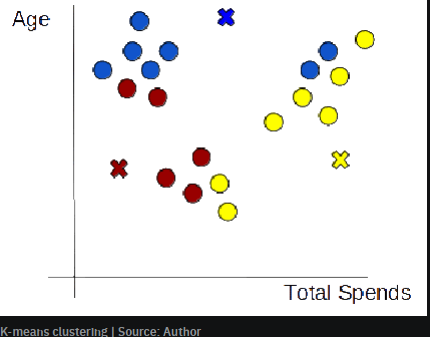
\includegraphics[width=0.5\linewidth]{K4.png}
    \caption{k4 Grupowanie K-średnich,dane przypisane do klastrów\cite{clust2020}}
\end{figure}
  
    D.  Zainicjuj ponownie centroidy
Następnie ponownie zainicjujemy centroidy, obliczając średnią wszystkich punktów danych tego klastra.


\begin{align*}
C_i = \frac{1}{\lvert N_i \rvert} \sum X_i
\end{align*}

Obliczamy centroide.Wzór\cite{clust2020}


\begin{figure}[!h]
    \label{fig:k6}
    \centering 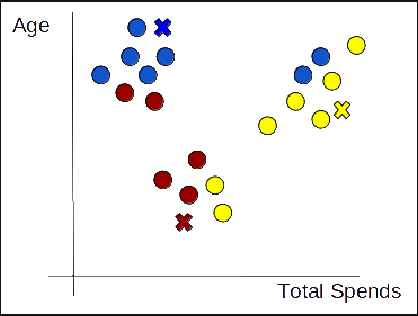
\includegraphics[width=0.6\linewidth,height=4cm]{K6.png}
    \caption{k6 Grupowanie K-średnich,dane przypisane do klastrów\cite{clust2020}}
\end{figure}
\newpage
     E.Powtórz kroki 3 i 4

Będziemy powtarzać kroki 3 i 4, aż uzyskamy optymalne centroidy, a przypisanie punktów danych do odpowiednich klastrów nie będzie się już zmieniać.
\begin{figure}[!h]
    \label{fig:k7}
    \centering 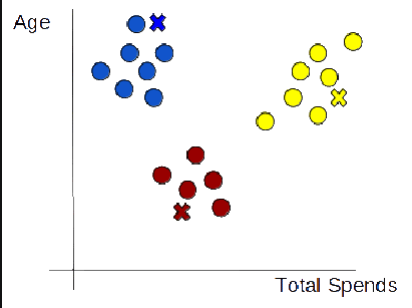
\includegraphics[width=0.5\linewidth, height=5cm]{K7.png}
    \caption{k7 Grupowanie K-średnich,dane przypisane do klastrów\cite{clust2020}}
\end{figure}

Does this iterative process sound familiar? Well, K-means follows the same approach as Expectation-Maximization(EM). \cite{clust2020}

\newpage


   
\newpage % Rozdziały zaczynamy od nowej strony.
\newpage
\section{Metodologia}
ma na celu przedstawienie dokładnego opisu metod i procedur, które zostały wykorzystane . pozwala innym zrozumieć, w jaki sposób przeprowadziłeś badanie i jakie kroki podjąłeś, aby uzyskać wyniki. 

\subsection{Gromadzenie i przygotowanie danych}
opisuje, skąd pochodzą dane badawcze, jak je zebrano i jak zostały przygotowane do analizy. Może to obejmować proces zbierania próbek, źródła danych, metody gromadzenia informacji, a także kroki konieczne do oczyszczenia i przetworzenia danych, takie jak usuwanie błędów czy brakujących wartości.

\subsection{Wybór algorytmu uczenia maszynowego:}
wyjaśniam, dlaczego wybrałem określone algorytmy uczenia maszynowego do rozwiązania mojego problemu. Opisuje, jakie kryteria były brane pod uwagę przy wyborze algorytmów i dlaczego one były odpowiednie dla  badania.

\subsection{Rozwój modelu}
opisuje kroki, które podjąłem w celu opracowania modelu uczenia maszynowego. To obejmuje wybór cech (feature selection), trenowanie modelu, dostrajanie parametrów, a także ewentualne eksperymenty i iteracje, które przeprowadziłeś, aby osiągnąć optymalne wyniki.


\subsection{Metryki oceny modelu}
wyjaśniam, jakie metryki i kryteria używam do oceny skuteczności modelu.



 
%\newpage % Rozdziały zaczynamy od nowej strony.
\section{Metodologia}
ma na celu przedstawienie dokładnego opisu metod i procedur, które zostały wykorzystane . pozwala innym zrozumieć, w jaki sposób przeprowadziłeś badanie i jakie kroki podjąłeś, aby uzyskać wyniki. 

\subsection{Gromadzenie i przygotowanie danych}
opisuje, skąd pochodzą dane badawcze, jak je zebrano i jak zostały przygotowane do analizy. Może to obejmować proces zbierania próbek, źródła danych, metody gromadzenia informacji, a także kroki konieczne do oczyszczenia i przetworzenia danych, takie jak usuwanie błędów czy brakujących wartości.

\subsection{Wybór algorytmu uczenia maszynowego:}
wyjaśniam, dlaczego wybrałem określone algorytmy uczenia maszynowego do rozwiązania mojego problemu. Opisuje, jakie kryteria były brane pod uwagę przy wyborze algorytmów i dlaczego one były odpowiednie dla  badania.

\subsection{Rozwój modelu}
opisuje kroki, które podjąłem w celu opracowania modelu uczenia maszynowego. To obejmuje wybór cech (feature selection), trenowanie modelu, dostrajanie parametrów, a także ewentualne eksperymenty i iteracje, które przeprowadziłeś, aby osiągnąć optymalne wyniki.


\subsection{Metryki oceny modelu}
wyjaśniam, jakie metryki i kryteria używam do oceny skuteczności modelu.
\newpage % Rozdziały zaczynamy od nowej strony.
\section{Studium przypadku}
przedstawiam konkretne przypadki lub scenariusze, w których zastosowano algorytmy uczenia maszynowego w kontekście zarządzania łańcuchem dostaw. Każda podsekcja jest poświęcona innemu przypadkowi z wykorzystaniem tych algorytmów. 

\subsection{Studium przypadku 1: Optymalizacja zapasów}
W tej sekcji przedstawiam konkretny scenariusz związany z zarządzaniem łańcuchem dostaw, gdzie wykorzystano algorytmy uczenia maszynowego do optymalizacji poziomu zapasów. Opisuje, jakie były cele tego studium przypadku, jakie dane zostały użyte do analizy oraz jakie algorytmy były stosowane w celu zoptymalizowania zarządzania zapasami.

\subsection{Studium przypadku 2: Prognozowanie popytu}
prezentuje konkretny przykład zastosowania algorytmów uczenia maszynowego do prognozowania popytu na produkty lub usługi w łańcuchu dostaw. Wyjaśniam, jakie były cele prognozowania popytu, jakie dane zostały użyte do tworzenia modeli prognozowania i jakie wyniki uzyskano w analizie.

\subsection{Studium przypadku 3: Wybór dostawcy}
Ta sekcja opisuje sytuację, w której algorytmy uczenia maszynowego zostały zastosowane do wyboru dostawcy w łańcuchu dostaw. Omawiam, jakie czynniki i kryteria były brane pod uwagę podczas procesu wyboru dostawcy, jakie dane były używane do analizy i jak algorytmy wspomagały w podjęciu decyzji.


\subsection{Studium przypadku 4: Planowanie produkcji}
W tej sekcji prezentuję przykład zastosowania algorytmów uczenia maszynowego do planowania produkcji w ramach zarządzania łańcuchem dostaw. Opisuję cele planowania produkcji, używane dane, a także wykorzystane algorytmy i techniki do optymalizacji procesów produkcyjnych.


\newpage % Rozdziały zaczynamy od nowej strony.
\section{Wyniki i dyskusja}
 prezentuje wyniki badań i analizuje ich znaczenie w kontekście zarządzania łańcuchem dostaw. 

\subsection{Porównanie wydajności algorytmów}
W tej sekcji dokonuje porównania wyników osiągniętych przez różne algorytmy uczenia maszynowego, które zostały użyte w Twoich studiach przypadku (lub w planowaniu produkcji). To pozwala na ocenę, który z algorytmów sprawdził się najlepiej w konkretnej sytuacji. Moge użyć różnych metryk oceny, aby porównać wydajność

\subsection{Interpretacja wyników}
W tej podsekcji analizuje i interpretuje wyniki uzyskane w badaniach przypadku . Wyjaśniasz, co otrzymane wyniki oznaczają w kontekście Twojego badania. Czy wyniki potwierdzają lub kwestionują pierwotne hipotezy lub cele? W jaki sposób algorytmy uczenia maszynowego wpłynęły na efektywność zarządzania łańcuchem dostaw lub planowania produkcji?

\subsection{Implikacje dla zarządzania łańcuchem dostaw}
W tej sekcji rozważam, jakie praktyczne implikacje wyników badań mają dla zarządzania łańcuchem dostaw. Jakie wnioski można wyciągnąć na temat optymalizacji procesów, efektywności czy podejmowania decyzji w łańcuchu dostaw na podstawie uzyskanych wyników? Jakie praktyczne zastosowania lub zalecenia można sformułować na podstawie  badań?


\newpage % Rozdziały zaczynamy od nowej strony.
\section{Wyniki i dyskusja}
 prezentuje wyniki badań i analizuje ich znaczenie w kontekście zarządzania łańcuchem dostaw. 

\subsection{Porównanie wydajności algorytmów}
W tej sekcji dokonuje porównania wyników osiągniętych przez różne algorytmy uczenia maszynowego, które zostały użyte w Twoich studiach przypadku (lub w planowaniu produkcji). To pozwala na ocenę, który z algorytmów sprawdził się najlepiej w konkretnej sytuacji. Moge użyć różnych metryk oceny, aby porównać wydajność

\subsection{Interpretacja wyników}
W tej podsekcji analizuje i interpretuje wyniki uzyskane w badaniach przypadku . Wyjaśniasz, co otrzymane wyniki oznaczają w kontekście Twojego badania. Czy wyniki potwierdzają lub kwestionują pierwotne hipotezy lub cele? W jaki sposób algorytmy uczenia maszynowego wpłynęły na efektywność zarządzania łańcuchem dostaw lub planowania produkcji?

\subsection{Implikacje dla zarządzania łańcuchem dostaw}
W tej sekcji rozważam, jakie praktyczne implikacje wyników badań mają dla zarządzania łańcuchem dostaw. Jakie wnioski można wyciągnąć na temat optymalizacji procesów, efektywności czy podejmowania decyzji w łańcuchu dostaw na podstawie uzyskanych wyników? Jakie praktyczne zastosowania lub zalecenia można sformułować na podstawie  badań?


\newpage % Rozdziały zaczynamy od nowej strony.
\section{Wniosek}
zakończenie pracy inżynierskiej i ma na celu podsumowanie kluczowych aspektów badania oraz przedstawienie ogólnych wniosków .

\subsection{Podsumowanie ustaleń}
W pierwszej części tej sekcji dokonuje podsumowania głównych ustaleń i wyników, które uzyskałem w trakcie swojego badania. To jest miejsce, gdzie można znaleźć najważniejsze informacje na temat  badania w jednym miejscu. Staram się podkreślić, co udało Ci się osiągnąć i jakie kluczowe wyniki uzyskałeś.

\subsection{Wkład}
 opisuje, jaki konkretny wkład praca wnosi do zarządzania łańcuchem dostaw i zastosowań uczenia maszynowego w SCM. Wyjaśniam, w jaki sposób badania rozwiązują istniejące problemy, rozwijają wiedzę lub otwierają nowe możliwości badawcze w tej dziedzinie. To jest miejsce, gdzie podkreślasz znaczenie pracy.

\subsection{Zastosowania praktyczne}
Omawiam praktyczne zastosowania wyników  badania w rzeczywistym środowisku biznesowym. Wyjaśniam, w jaki sposób przedsiębiorstwa lub organizacje mogą wykorzystać  ustalenia i techniki w praktyce. To pozwala  zrozumieć, jakie korzyści mogą wyniknąć z mojej pracy dla przemysłu i sektora SCM.

\subsection{Wnioski i uwagi końcowe}
W tej ostatniej części pracy podkreślam główne wnioski i formułuje uwagi końcowe na temat całego procesu badawczego. podziękowania za wsparcie, podsumowania, dlaczego ta praca jest istotna i jakie znaczenie ma dla dziedziny zarządzania łańcuchem dostaw oraz zastosowań uczenia maszynowego w SCM.
\newpage % Rozdziały zaczynamy od nowej strony.
\section{Wniosek}
zakończenie pracy inżynierskiej i ma na celu podsumowanie kluczowych aspektów badania oraz przedstawienie ogólnych wniosków .

\subsection{Podsumowanie ustaleń}
W pierwszej części tej sekcji dokonuje podsumowania głównych ustaleń i wyników, które uzyskałem w trakcie swojego badania. To jest miejsce, gdzie można znaleźć najważniejsze informacje na temat  badania w jednym miejscu. Staram się podkreślić, co udało Ci się osiągnąć i jakie kluczowe wyniki uzyskałeś.

\subsection{Wkład}
 opisuje, jaki konkretny wkład praca wnosi do zarządzania łańcuchem dostaw i zastosowań uczenia maszynowego w SCM. Wyjaśniam, w jaki sposób badania rozwiązują istniejące problemy, rozwijają wiedzę lub otwierają nowe możliwości badawcze w tej dziedzinie. To jest miejsce, gdzie podkreślasz znaczenie pracy.

\subsection{Zastosowania praktyczne}
Omawiam praktyczne zastosowania wyników  badania w rzeczywistym środowisku biznesowym. Wyjaśniam, w jaki sposób przedsiębiorstwa lub organizacje mogą wykorzystać  ustalenia i techniki w praktyce. To pozwala  zrozumieć, jakie korzyści mogą wyniknąć z mojej pracy dla przemysłu i sektora SCM.

\subsection{Wnioski i uwagi końcowe}
W tej ostatniej części pracy podkreślam główne wnioski i formułuje uwagi końcowe na temat całego procesu badawczego. podziękowania za wsparcie, podsumowania, dlaczego ta praca jest istotna i jakie znaczenie ma dla dziedziny zarządzania łańcuchem dostaw oraz zastosowań uczenia maszynowego w SCM.


%\newpage % Rozdziały zaczynamy od nowej strony
%\section{Podsumowanie}          % Można też pisać rozdziały w jednym pliku.
%\lipsum[5-10]

%--------------------------------------------
% Literatura
%--------------------------------------------
\cleardoublepage % Zaczynamy od nieparzystej strony
\printbibliography

%--------------------------------------------
% Spisy (opcjonalne)
%--------------------------------------------
\newpage
\pagestyle{plain}


\vspace{0.8cm}
\acronymlist
\acronym{EiTI}{Wydział Elektroniki i Technik Informacyjnych}
\acronym{PW}{Politechnika Warszawska}
\acronym{WEIRD}{ang. \emph{Western, Educated, Industrialized, Rich and Democratic}}

\listoffigurestoc     % Spis rysunków.
\vspace{1cm}          % vertical space
\listoftablestoc      % Spis tabel.
\vspace{1cm}          % vertical space
\listofappendicestoc  % Spis załączników

% Załączniki
\newpage
\appendix{Nazwa załącznika 1}
COS TAM TAM  COS TAM

\newpage
\appendix{Nazwa załącznika 2}
COS TAM TAM  COS TAM



\end{document} 
